\chapter{Synthesis of Past Research}\label{ch:synthesis-of-past-research}


\section{Overview}\label{sec:overview}

In the last decade and more I have worked on a diverse range of projects and problems. These problems are woven together by a desire to understand how the Earth works from observations. Generally, my research sits in two categories: mantle processes and surface processes. In some cases, notably work I did in collaboration with Rob Duller and Stefan Schmalholz in 2014 \citep{armitage-etal-2014}, and a collaboration with Miguel Andrés-Mart\'inez, Marta Pérez-Gussinyé, and Jason Morgan \citep{andres-martinez-etal-2019}, these two areas have combined, and we have looked at the connectivity between surface processes and the upper mantle. In this Chapter I will however focus on the two areas as separate cases, and bring forward my overall aim, which is to use observations to build an understanding of the processes at play. At the end of the thesis there are two annexes. In Annex A I include five example publications that focus on mantle processes, and in Annex B I include five example publications that focus on surface processes. These publications expand and compliment the summary of my past research.

There is one notable omission in this synthesis of my research, that I want to mention up front: intracratonic basins. These long-lived and exceptionally dull sedimentary basins exist across every continent, including the well known Paris Basin. With Philip Allen, I developed a theory for how they form: by exceptionally slow and long-lived extension \citep{armitage-2010,allen-2012}. Subsequently with Claude Jaupart, Loïc Fourel, and Francis Lucazeau we explored how subsidence within these basins is further modified by convective instabilities at the margins of continental lithsophere \citep{armitage-etal-jgr-2013,lucazeau-etal-2015}. Intracratonic basins, while being a favourite of mine, do not form part of this thesis and shall not appear in the story developed below.

\section{Mantle Processes}

Observations from seismic arrivals and rock geochemistry have, for decades, been used to infer mantle conditions both at large depths and throughout the Earth's history. Below regions of active volcanism, such as the East Pacific Rise, La Réunion or Afar, Africa, there are regions of slow seismic velocity \citep[e.g.][]{forsyth-etal-1998,mazzullo-etal-2017,bastow-etal-2005}. Such regions of low seismic velocity can be interpreted to be due to increased mantle temperature relative to the background and the retention of melt within the rock matrix \citep[e.g.][]{goes-etal-2012,armitage-etal-epsl-2015}. The first region that lead to the hypothesis that significant melt, 2\,\% porosity, is stored within the mantle was the East Pacific Rise. From the MELT and GLIMPSE passive seismic experiments, the best fitting inverse models mapped a region with 11\,\% lower seismic velocities compared to the global average. The argument is that such a low seismic velocity canot be achieved by thermal effects alone, and the only way to reduce the velocity further is the storage of partial melt \citep{harmon-etal-2009}. This argument is likewise used when interpreting inverse models of seimsic arrivals below the East African rift \citep[e.g.][]{gallacher-etal-2016,chambers-etal-2019}, where up to 2\,\% porosity is estimated for below the Main Ethiopian Rift \citep{chambers-etal-2019}. 

The hypothesis that there is relatively high melt retention in mantle has implications on what defines the seismic discontinuities away from regions of volcansim. The lithosphere asthenosphere boundary (LAB) is a seismically imaged contrast or discontinuity that is found at various depths through the continental and oceanic lithosphere. In the oceanic lithosphere it has been proposed to map the depth at which retained melt gets frozen into mantle \citep[e.g.][]{hirschmann-2010,mehouachi-2017}. However, the LAB could also reflect a change in the dominant deformation mechanism in the mantle \citep[e.g.][]{karato-2012,goes-etal-2012,beghein-etal-2019}.

The continual interpretation of low seismic velocities from inverse models as being due to high melt retention is at odds with melt chemistry. From the decay of isotopes, it is estimated that melt transport is rapid \citep[e.g.][]{elliot-2014}. If melt is efficiently transported from the zone of partial melting to the surface then large quantities cannot be retained within the mantle and other factors must lead to the low velocities that are required to fit the seismic arrivals. For example below the East Pacific Rise, it has been demonstrated that the effects of attenuation of seismic waves due to thermal effects is sufficient to explain the 11\,\% drop in seismic velocities without the need to invoke retention of melt \citep{goes-etal-2012}.

The use of geodynamic models to test interpretations from inverse models, as exemplified in \cite{goes-etal-2012}, is one of the key aspects of my research that I will now focus on. I have worked on six key geological regions: the North Atlantic volcanic margins, the South Atlantic volcanic margins, the India-Seychelles margins, the East African Rift, Icelandic volcanism, and La Réunion. The first four regions were previously summarised in \cite{armitage-2018} (see Figure\ref{fg:4models}). Here I will update the discussion on Afar based on more recent publications, and add recent work on Iceland and La Réunion. In each of these regions I have developed forward models of the geophysical processes that lead to decompression melting and compared them with the observations (for a description of the basic model equations see Appendix \ref{app1}). This allows for hypotheses based on the interpretation of inverse models and rock chemistry to be robustly tested, leading to a better understanding of the mantle structure.

\subsection{East African Rift}

\begin{sidewaysfigure}
\centering
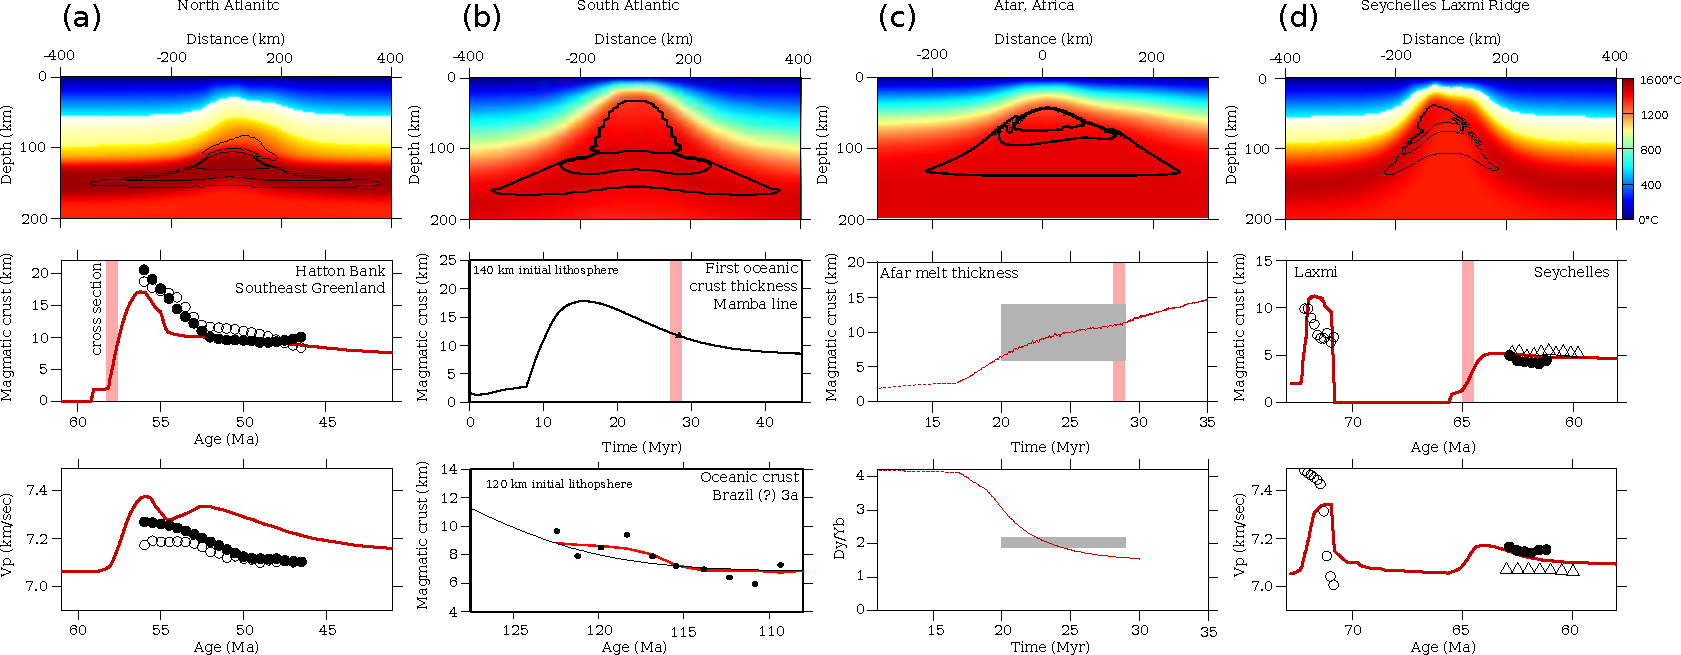
\includegraphics[width=22.5cm]{./figures/ch2-mantle2.pdf}
\caption{Key model results for four study areas \citep[see][]{armitage-2018}. The top figures show the thermal conditions within the model at the time step shown by the pink bar in the lower diagrams. The black outlines show the regions that are producing melt with contours representing 1\,\% (long dashed lines) and 2\,\% (short dashed lines) melting. The lower figures show examples of observations (symbols or in the Afar case a grey box) compared to model predictions (red lines). We have chosen to show models from early stage of rifting (North and South Atlantic) and from late stage (South Atlantic and Afar). In the former two examples there are rift jumps, hence the melt area shown is asymmetric. There is no other significance to the choice of time step for each location. (a) North Atlantic: the lithosphere has been pre-stretched by the formation of the Hatton Trough at $5\rm\,mm\,yr^{-1}$ \citep[see][]{armitage-etal-2009}, and subsequently the event that leads to break-up at a half spreading rate that is initially $40\rm\,mm\,yr^{-1}$ and reduces to $10\rm\,mm\,yr^{-1}$ at 55\,Ma. The model is compared to estimates of the thickness and $V_{p}$ of igneous intrusions from the SIGMA-3 -- iSIMM Hatton Bank conjugate margins \citep{hopper-etal-2003,white-etal-2008}. (b) South Atlantic: the lithosphere has been stretched in one phase at a half spreading rate of $14\rm\,mm\,yr^{-1}$ \citep[see][]{taposeea-etal-2016}. The model is compared to the thickness of the oceanic crust offshore Namibia (Mamba line) and Pelotas (ION-GX). (c) India–Seychelles: the lithosphere has been stretched in two phases, first the formation of the Gop Rift at a half spreading rate of $80\rm\,mm\,yr^{-1}$, followed by extension between the Seychelles and Laxmi Ridge at a half spreading rate of $60\rm\,mm\,yr^{-1}$ \citep[see][]{armitage-etal-g3-2011}. The model is compared to estimates of the thickness and P-wave seismic velocity ($V_{p}$) of igneous intrusions from both margins \citep{collier-etal-2009,minshull-etal-2008}. (d) Afar, Africa: the lithosphere has been stretched in two phases, first due to the formation of the southernmost Red Sea at $5\rm\,mm\,yr^{-1}$, and then within Afar at a half spreading rate of $7\rm\,mm\,yr^{-1}$ \citep[see][]{armitage-etal-2015}. The model is compared the estimates of the thickness of the igneous crust and the Dy/Yb ratio of melts erupted.}
\label{fg:4models}
\end{sidewaysfigure}

\begin{figure}
    \centering
    \includegraphics[width=12cm]{./figures/ch2-EAR.png}
    \caption{(a) The East African Rift region comprising the Afar region, the Main Ethiopian Rift (MER), and eastern and western branches (EB, WB) south of the study area (red box). Orange triangles represent Holocene volcanoes. Brown lines delineate active fault zones. (b) Horizontal slice at 500 km depth through the undamped P model, NEAR-P15. The black line indicates the orientation of the cross sections in (c) and (d). (c) Vertical cross section through the undamped NEAR-P15. (d) Vertical cross section through the undamped NEAR-S16. The cross section reveals two clusters of low-velocity anomalies below Afar and MER extending down to the base of the transition zone. Figure from \cite{civiero-etal-2019}.}
    \label{fg:EAR}
\end{figure}

\subsubsection*{Upper mantle structure}

The seismic velocity found in inverse models of the mantle below the Northern East African Rift (EAR) is spectacularly low (Figure \ref{fg:EAR}). This coupled with the chemistry of lavas erupted would suggest that there is a source of very hot mantle below this young rift zone. Classic tomographic models for the mantle below Africa have suggested that there is a broad low-velocity layer present through the whole upper mantle beneath the EAR, and this is interpreted to be a large-scale upwelling named the African Superplume \citep[e.g.][]{ritsema-etal-1999}. As the number of seismometers deployed within Africa has increased the resolution of tomographic images has increased. It is now thought that this structure is potentially multiple smaller-scale features and not one large upwelling \citep{chang-2011,hammond-etal-2013,civiero-etal-2015,emry-etal-2019}. This complexity is not unique to the African structure, below Iceland the low-velocity anomaly is a complex branching structure \citep{rickers-etal-2013}, the Azores, Canary and Cape Verde low-velocity zones may be linked \citep{saki-etal-2015}, and likewise for structures below the Iberian peninsular and Maghreb \citep{civiero-etal-2018}. These interpretations lead to the suggestion that there exist secondary plumes rising below zones of active volcanism, as for example observed within laboratory experiments \citep{davaille-2005,kumagai-etal-2007}.

Secondary plumes, such as those within the experiments of \cite{kumagai-etal-2007}, arise due the stagnation of the main plume head. In the Earth such stagnation could be due to density changes because of endothermic phase transitions at the 660\,km discontinuity \citep[e.g.][]{tosi-2011,bossmann-2013}. The stagnated material heats up the boundary at the 660\,km discontinuity and generates new plumes at a smaller scale, which would have a spacing of the order of hundreds of kilometers. This scaling argument lead to the hypothesis that the structures seen in the inverse models from seismic arrivals are due to such small-scale plumes \citep{civiero-etal-2015}. In collaboration with Chiara Civiero and Saskia Goes, we tested this hypothesis. The goal was to use a similar approach to earlier work on the EAR and the East Pacific Rise \citep{armitage-etal-2015,goes-etal-2012}:
\begin{itemize}
\item[1] Develop a forward model of the geodynamic processes in three dimensions at a scale similar to the EAR.
\item[2] Convert the physical model properties to seismic velocities, taking into account the effects of attenuation.
\item[3] Resolve the numerical model at the same resolution as the tomographic models. This means using the numerical model as an input model for the inversion and observing how the high resolution image gets damped and smoothed due to the resolution of the seismic array.
\end{itemize}

\begin{figure}
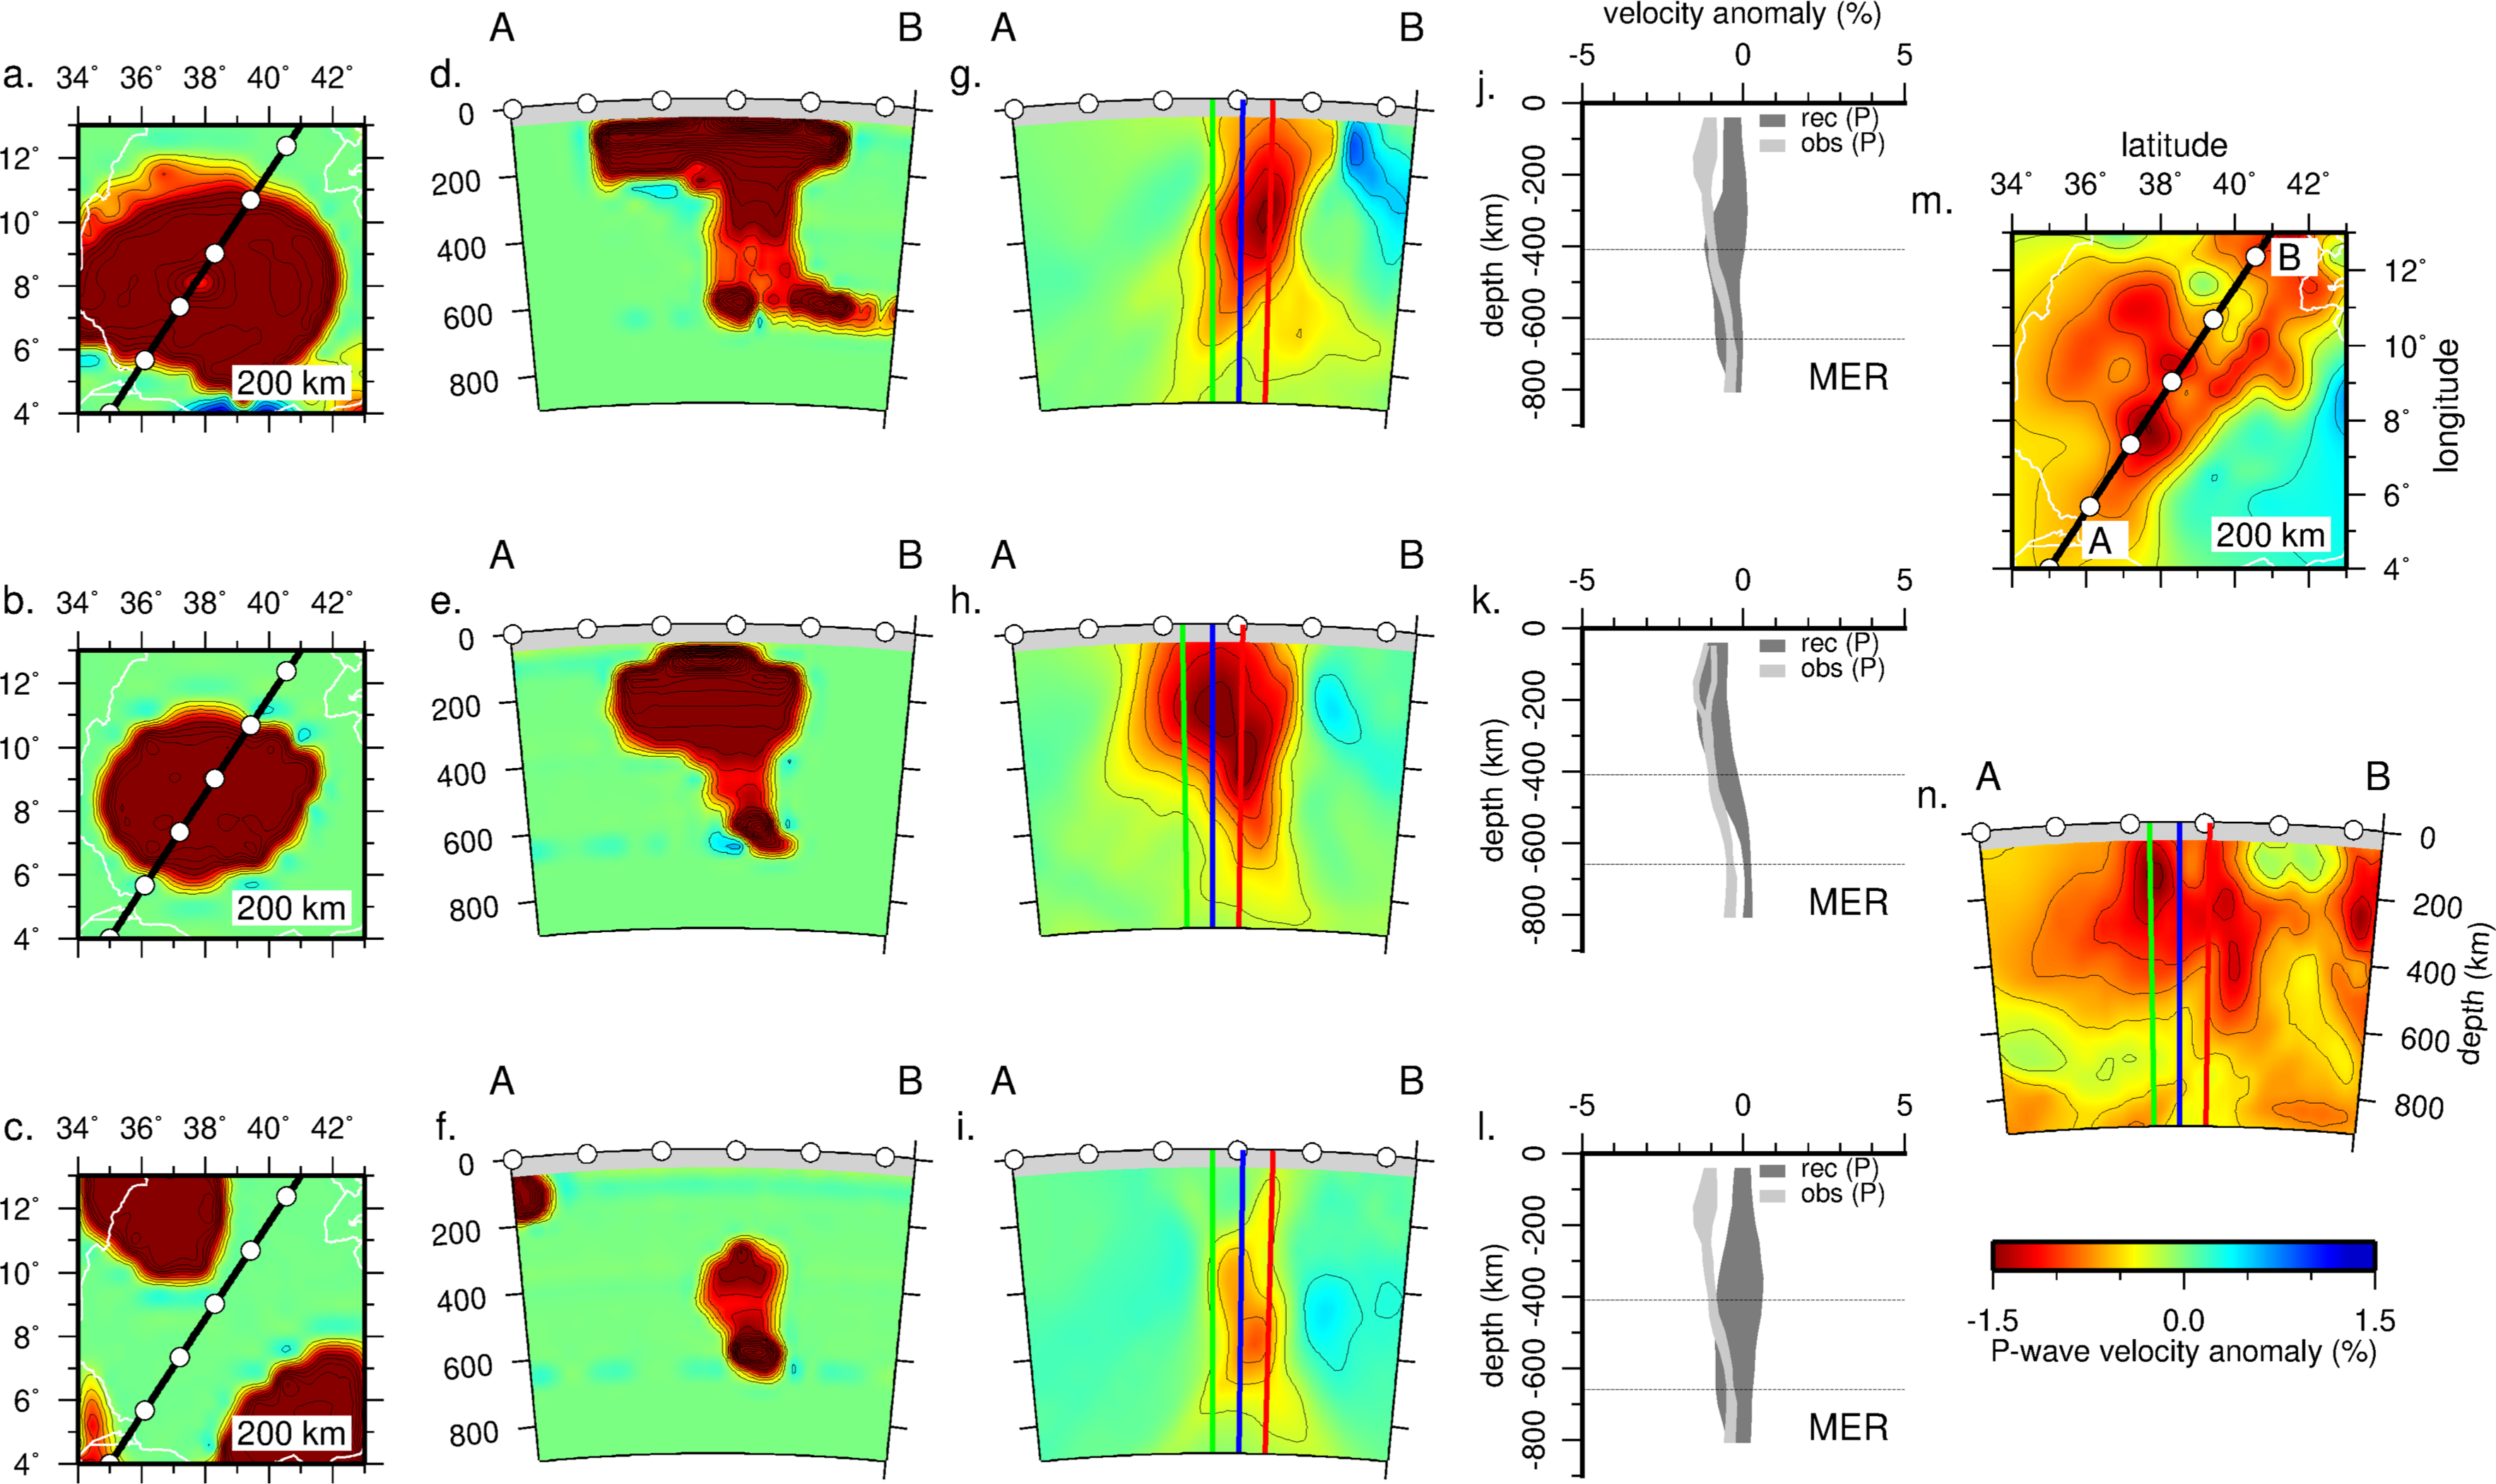
\includegraphics[width=\textwidth]{./figures/ch2-tomography.png}
\caption{Figure from \cite{civiero-etal-2019}: Horizontal slices and vertical cross sections through the P wave from the destabilisation of a layer with an excess temperature of $200\rm\,^{\circ}C$ (Rayleigh Taylor instability), focused below the Main Ethiopian Rift. The orientation of the cross sections (black line) is shown in each 200 km depth slice. (a-c) Horizontal slices at 200 km depth through the synthetic models of LS (a), MS (b), and ES (c) phases. (d, g) Synthetic and resolved images of the LS plume phase; (e, h) synthetic and resolved images of the MS plume phase; (f, i) synthetic and resolved images of the ES plume phase. The resolved LS plume (g) lost its head due to the lack of resolution at shallow upper-mantle depths. The MS phase (h) is well resolved because the head of the input model (b) is relatively strong and laterally confined. Although some smearing, the ES structure (i) is quite well recovered. (j-l) Input and retrieved P wave velocity anomaly envelopes (\%) along the green, blue, and red profiles drawn in the cross sections. Within the transition zone the retrieved and observed velocity anomalies of the MS and LS plumes overlap. (m) The 200 km depth slice through the NEAR-P15 model. (n) Vertical cross section through the NEAR-P15 model. The spacing between the contours is 0.25\,\%. White points indicate the distance every $2\rm\,^{\circ}$ . The color scale is the same for all the panels.}
\label{fg:EAR-plumes}
\end{figure}

We explored two possibilities, first that the small-scale plumes are like Rayleigh Bénard convection cells and secondly that they are due to the destabilisation of ponded plume material (Rayleigh Taylor instabilities). In total 10 model setups were explored with additional variations to the assumed mantle rheology, initial thermal structure and boundary conditions, and model aspect ratio (see \citealp{civiero-etal-2019} for the full details). By converting the numerical model to synthetic tomographic images it was quickly found that the thermal structure of the small-scale plumes had to create a significant and sharp contrast in seismic velocity. Simple Rayleigh Bénard convection created plumes that were either too thin (for a non-Newtonian rheology) or were too diffuse (for a Newtonian rheology), such that the synthetic tomography did not recover the strong contrast in seismic velocity seen in the inversion \citep{civiero-etal-2019}.

The only models that could recreate the contrast in seismic velocity within the inversions were those that looked at the Rayleigh Taylor-like destabilisation of a layer of hot material that was initially at the base of the model domain at between 600 and 700\,km (Figure \ref{fg:EAR-plumes}). This layer rises upwards as plume-like structures with a spacing that is similar to the the spacing in the tomographic models (Figure \ref{fg:EAR-plumes}). The implication is that below the EAR mantle material stagnated below the 660\,km discontinuity due to mineral phase changes. Rather than this ponded material heating the upper mantle and creating secondary plumes, the ponded material became buoyant and rose into the upper mantle as a Rayleigh Taylor instability giving rise to the distribution of volcanism we observe today in the EAR. A mechanism that could lead to such behaviour is internal heating, which would cause a stagnated plume head to become thermally buoyant over time and destabilise. This could be tested in future laboratory experiments \citep[e.g.][]{limare-etal-2019}.

One important point that comes from this work is that the interpretation that the patterns seen in the seismic tomography are due to small-scale plumes is overly simplistic. There is a need to go further and explore if such interpretations are possible. Secondary plumes due to a thermal boundary layer at the 660\,km discontinuity cannot create the observed magnitudes of low velocities. Instead, the only model that can match the magnitude of the seismic velocity anomalies requires that material passes through the boundary between the upper and lower mantle (Figure \ref{fg:EAR-plumes}). Beyond trying to understand how the deep Earth functions, this research has wider implications to how we practice seismology. The interpretation of an inverse model is not an observation nor a result. Seismological studies should not end with an interpretation of the preferred inversion. Rather, these interpretations should be posed as hypotheses that can be tested. We can resolve numerical models at the resolution of seismic deployments \citep[e.g.][]{goes-etal-2012,civiero-etal-2019}, and by doing so discover if the hypothesis stack up against the seismic data.

\subsubsection*{Lithosphere structure}

At a shallower scale, from an inverse model based on receiver functions and Rayleigh waves, it was interpreted that the crust and mantle lithosphere are decoupled below the Main Ethiopian Rift \citep{keranen-etal-2009}. It was thought that the seismic velocities required by the inverse model are indicative of a hot and therefore weak lower lithosphere. Narrow rifting in the Main Ethiopian Rift was therefore due to pre-existing structural controls in the crust, and not due to the integrated strength of the lithosphere \citep{keranen-etal-2009}. However, the width of the region of extension has been shown, numerically, to depend on the rhoelogical laws chosen for the crust and lithosphere \citep[e.g.][]{buck-1991,brun-1999,brune-etal-2017}. Furthermore, the timing of the onset of volcanism is affected by the crustal strength within numerical models \citep{ros-etal-2017}. Therefore, it is possible that the structure of early rifting in the northern East African Rift is due to crustal rheology rather than an unknown inheritance. Importantly, the interpretation from the seismic data can be treated as a hypothesis and tested using numerical models of our best understanding of the physics behind the deformation of the upper mantle.

In collaboration with Kenni Petersen, we developed a 2D model of visco-elasto-plastic deformation of the upper mantle (MESS\footnote{MESS: Multigrid Elastic and Stuff Solver (or Multigrid Elasto-plastic-viscous Strain Solver), see \url{https://bitbucket.org/johnjarmitage/mess}}) that includes melting and in particular the prediction of melt composition \citep{petersen-etal-2015,armitage-etal-g3-2018}. By varying the strength of the crust we showed that evolution of the depletion of lavas in light trace elements is a function of the strength of the crust. When the crust is strong, it thins rapidly and extension localises creating a narrow rift. This is analogous to there being only a thin lithospheric lid on top of the zone of partial melting. This thin lid does not suppress the development of a `triangular' zone of partial melting (as shown in Figures \ref{fg:melt-region} and \ref{fg:4models}). The result is that light trace elements, such as lanthanum, are depleted rapidly with respect to heavier trace elements, such as ytterbium. If however the crust is weak, extension is not localised and a thicker lithospheric lid rests upon the zone of partial melting. This results in a slower reduction in light relative to heavy trace elements within the erupted lava \citep{armitage-etal-g3-2018}.

\begin{figure}
\centering
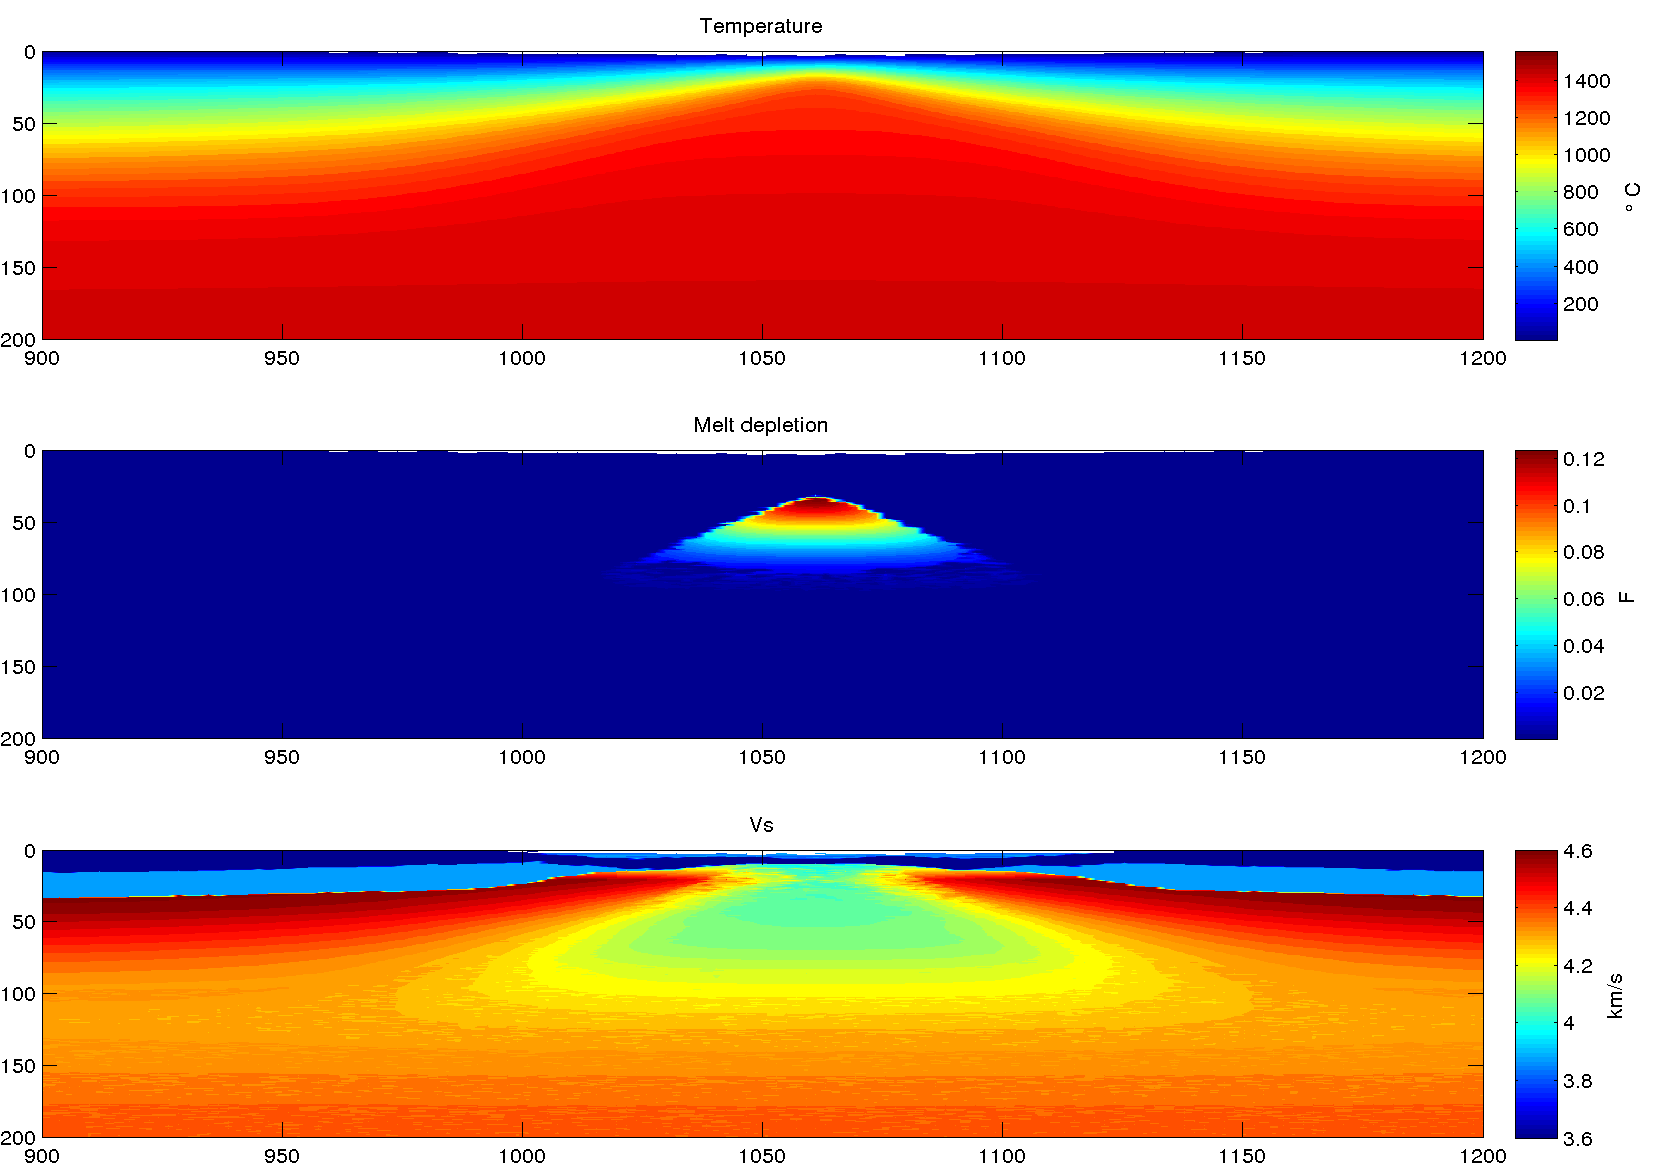
\includegraphics[width=\textwidth]{./figures/ch2-mantleVs.pdf}
\caption{Predicted thermal structure, melt depletion, and S-wave seismic velocity after 25 Myr of extension for with an extension rate of $5\rm\,mm\,yr{-1}$ and mantle potential temperature of $1350\rm\,^{\circ}C$. (a) Temperature, (b) melt fraction, and (c) S-wave seismic velocity. Figure taken from \cite{armitage-etal-g3-2018}.}
\label{fg:mantleVs}
\end{figure} 

When this model was applied to the Main Ethiopian Rift it was found that in order to recreate the observed lava chemistry, only a model with a strong crust could achieve sufficient melt generation. Furthermore, when the predicted upper mantle structure was converted to S-wave velocity (Figure \ref{fg:mantleVs}), it was found that the model velocities were within the range of the observed 1D inversions (Figure \ref{fg:MER-Vs} black line). The hypothesis that breakup in the Main Ethiopian Rift is defined by the extension of a weak lithosphere does not match the observations \citep[c.f.][]{keranen-etal-2009}. The numerical model that best fits the data is of a strong lithosphere. This once more demonstrates that hypotheses, or \emph{interpretations}, based from inverse seismic models can be tested with forward numerical models.

For shallower depths the forward model does not match the low seismic velocities required by the inversion (Figure \ref{fg:mantleVs}). However, if it is assumed that 1\,\% melt is stored within the lithosphere above a depth of 40\,km, then the shallow structure can be even better explained. The 2D code MESS does not include melt transport (e.g.\ equation \ref{eq:mass-melt} in Appendix \ref{app1}) and therefore the hypothesis that there is significant melt storage within the uppermost lithosphere below the Main Ethiopian Rift was not explored. However, as developed in the following section, this aspect could be incorporated in future studies.

\begin{figure}
\centering
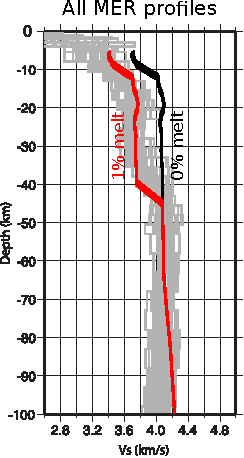
\includegraphics[width=4cm]{./figures/ch2-MER-Vs.pdf}
\caption{Comparison of the predicted S-wave seismic velocity from the for-ward model with a strong lower crust (Figure \ref{fg:mantleVs}c), and the ensemble vertical profiles from the joint inversion of Rayleigh waves and receiver functions below the Main Ethiopian Rift \citep{keranen-etal-2009}. The black line is the model $V_{S}$ assuming no melt storage, the red line assumes that 1\,\% melt is stored above 40\,km depth.}
\label{fg:MER-Vs}
\end{figure}

\subsection{Iceland}

\begin{figure}
\centering
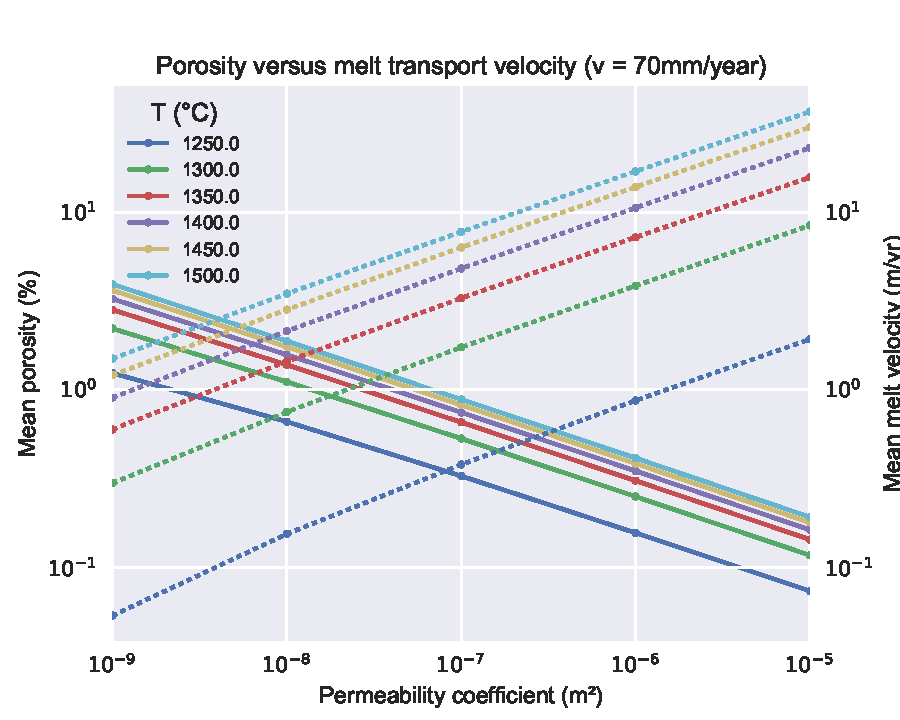
\includegraphics[width=8.6cm]{figures/ch2-phi-vm.pdf}
\caption{Logarithmic plot of the variation in modelled porosity (solid) and melt flow velocity (dashed) with permeability coefficient and temperature, with up-welling velocity constant at $70\rm\,mm\,yr^{-1}$. The relationship between porosity and mean melt flow velocity is inversely proportional as a function of the permeability coefficient, and proportional as a function of temperature. Figure is from \cite{franken-etal-2020}.}
\label{fg:phi-vm}
\end{figure}

The retention of melt within the upper mantle, as invoked at the end of the last section, has been cited as causing seismic discontinuities and regions of low velocity observed below volcanic islands, rift zones, and mid-ocean ridges \citep[e.g.][]{forsyth-etal-1998,harmon-etal-2009,rychert-etal-2012,rychert-etal-2014}. Typical estimates of the quantity of melt range from 0.1\,\% to 2\,\%. The low seismic velocities below Iceland can be explained by the presence of high temperatures but discontinuities required by receiver function inversions would require an extra $\sim 1$\,\% melt \citep{rychert-etal-2018}. High melt retention would naturally imply low melt velocities and low permeability (Figure \ref{fg:phi-vm}; \citealp{weatherley-2016,franken-etal-2020}). However, forward modelling of decompression melting below both the East Pacific Rise and Afar (Figure \ref{fg:4models}c; \citealp{goes-etal-2012,armitage-etal-2015}), suggest that high melt retention, $>0.5$\,\% is unlikely. 

The glaciers on Iceland have been reducing in size since the last glacial maximum. Iceland experienced a rapid deglaciation around ten thousand years ago (Figure \ref{fg:iceland-map}). The rapid depressurisation of the upper mantle due to this loss in surface load could lead to an significant increase in decompression melting \citep{jull-1996}. This is in line with outcrop evidence of the volume and composition of lava erupted since the late-Pleistocene \citep{maclennan-etal-2002,sinton-etal-2005,eksinchol-etal-2019}. However, if the observed change in lava composition and volume estimates were caused by deglaciation, the transport of melt from the zone of partial melting to the surface must be rapid, and rapid melt transport implies low melt retention (Figure \ref{fg:phi-vm}). This is therefore again at odds with the interpretation of high melt retention derived from seismic inversions.

\begin{figure}
\centering
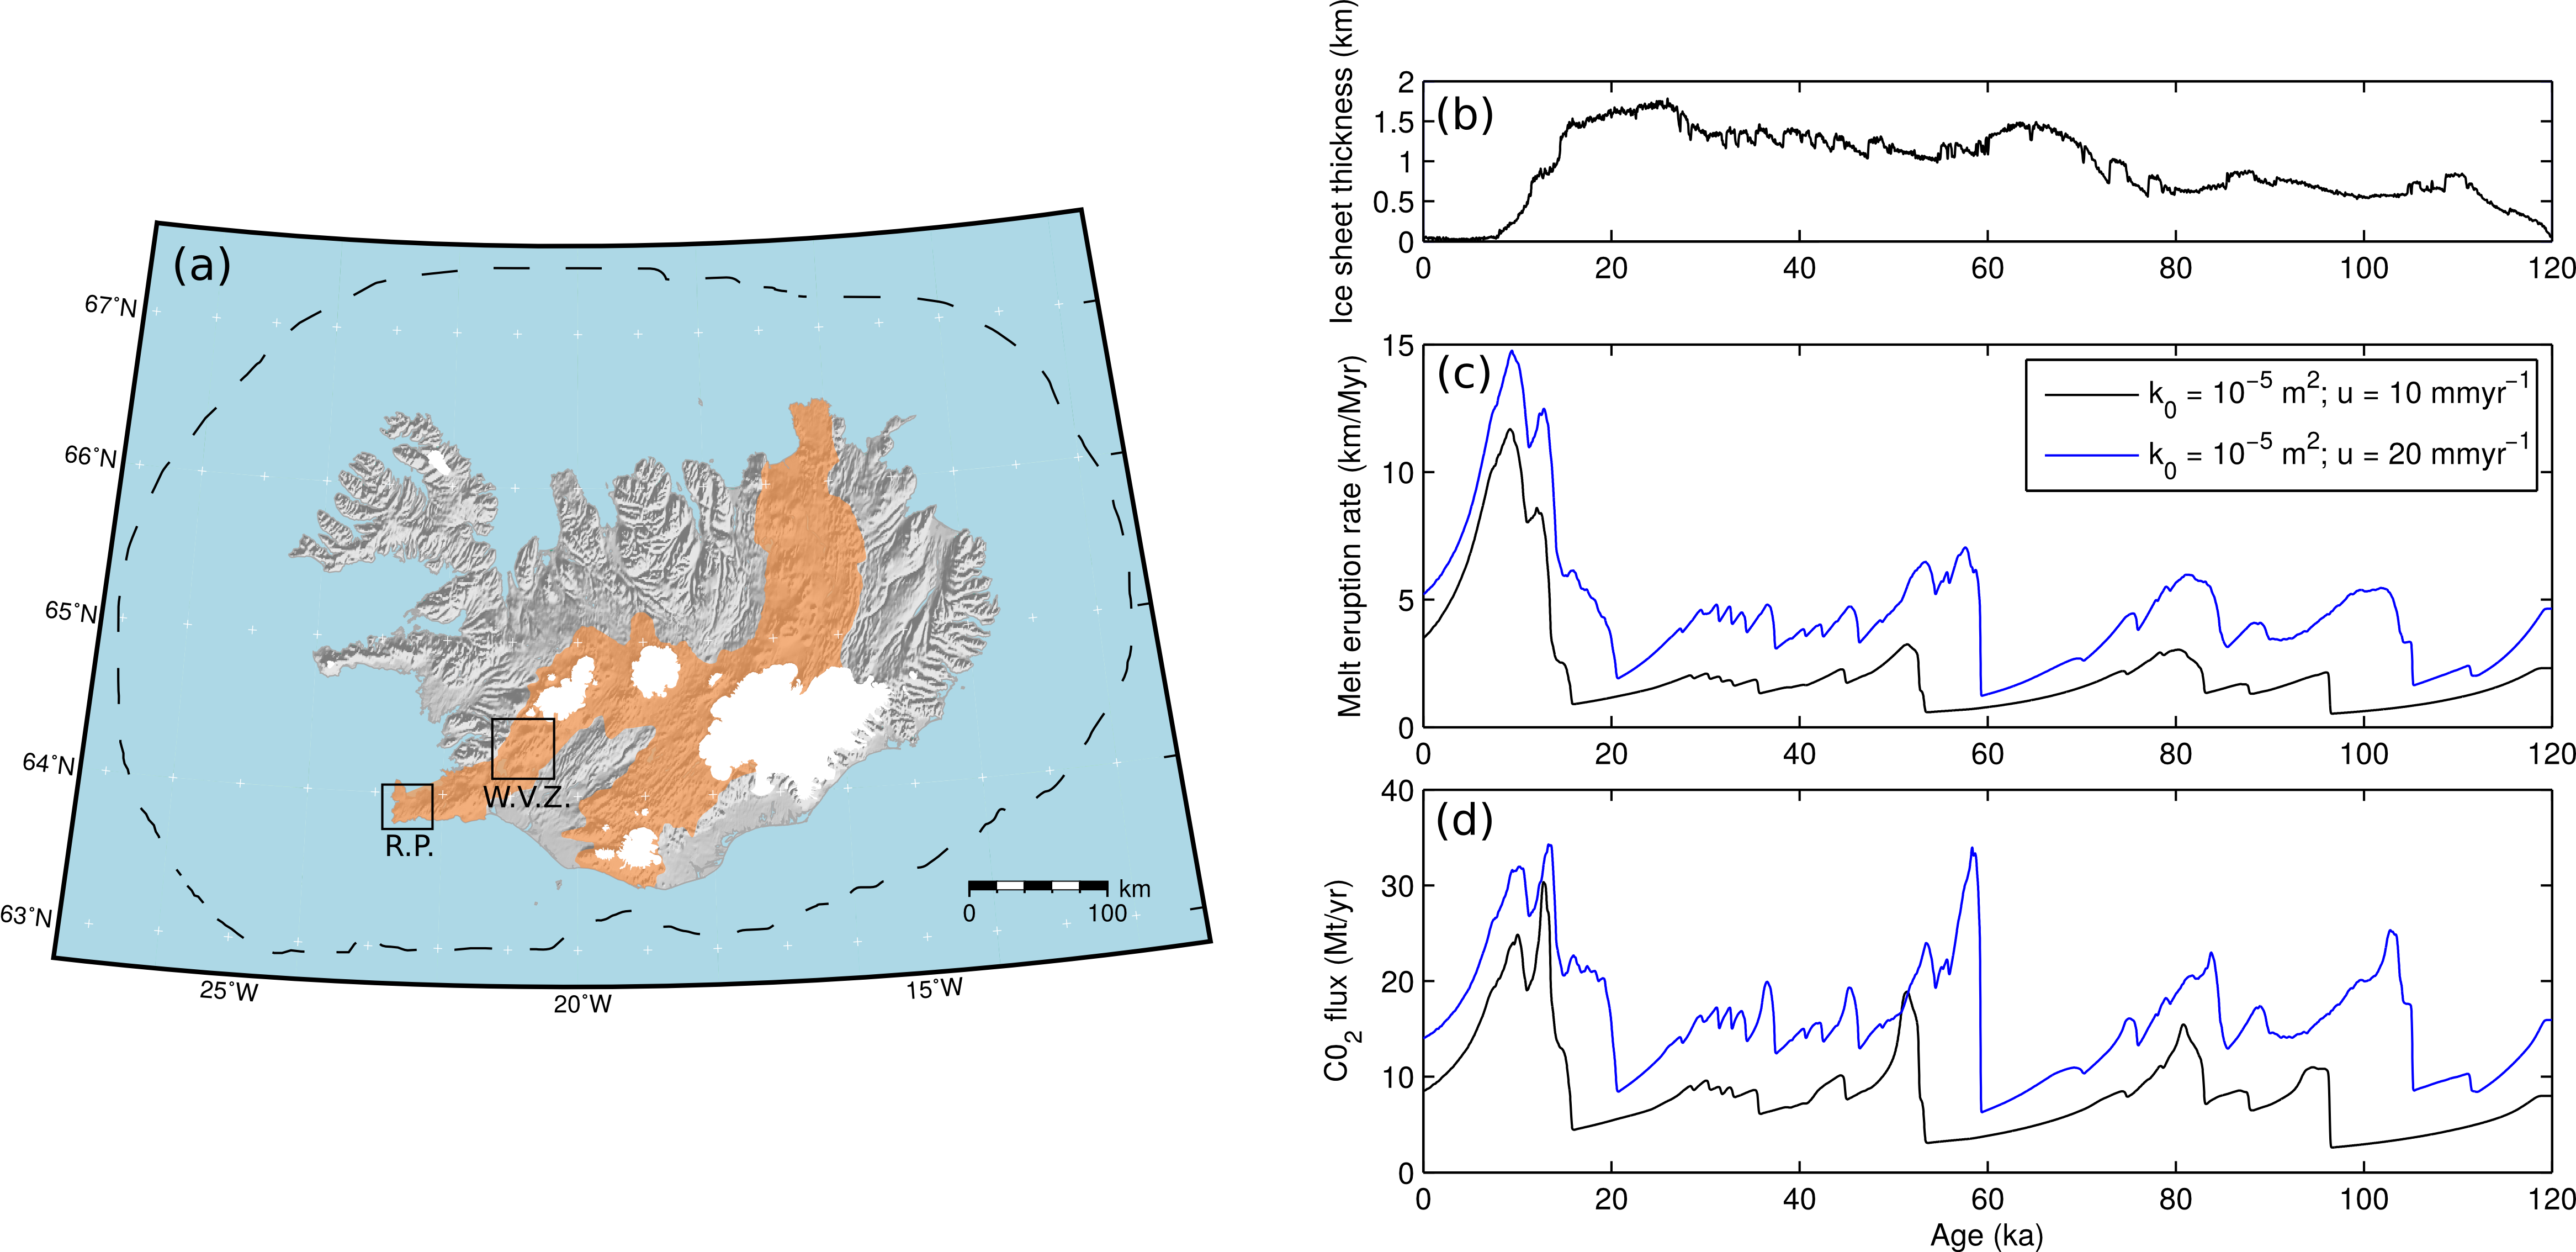
\includegraphics[width=\textwidth]{./figures/ch2-iceland-map.png}
\caption{Response of the model to periodic and observed ice sheet thickness changes of the last 120\,ka. (a) Map of Iceland showing the locations of the volcanic rift zones in orange and the maximum extent of the ice sheet at the last glacial maximum (dashed line). The boxes show the location of the Reykjanes Peninsular (R. P.) and the Western Volcanic Zone (W. V. Z.). (b) The ice sheet thickness predicted from the ice sheet model M1 over the last 120\,ka. (c) Melt eruption rate and (d) carbon flux response to the step change in ice sheet thickness: black line, an upper mantle permeability coefficient of $k_{0} = 10^{-5}\rm\,m^{2}$ and up-welling velocity of $10\rm\,mm\,yr^{-1}$, and blue line, an up-welling velocity of $20\rm\,mm\,yr^{-1}$.}
\label{fg:iceland-map}
\end{figure}

To understand if the observed change in lava composition is due to deglaciation I worked with Kenni Petersen, David Freguson, and Tim Creyts, to create a 120\,kyr history of ice sheet growth and decay on Iceland (Figure \ref{fg:iceland-map}b) and develop a 1D model\footnote{The 1D model can be found at: \url{https://bitbucket.com/johnjarmitage/melt1d-icesheet/}} that can predict eruption rates, lava compositions, and melt retention as the surface load changes \citep{armitage-etal-grl-2019}. From exploring the physically plausible parameter space, we found that deglaciation would indeed impact lava eruption rates if the mantle permeability is high (Figure \ref{fg:iceland-map}c and d). In order to recover a system response that matched the estimated eruption rates from outcrops, and the observed neodymium (Nd) concentrations the permeability of the mantle $k_{\phi} = k_{0}\phi$ needs to be on the order of $10^{-14}\rm\,m^{-2}$, melt retention of $\sim 0.1$\,\% \citep{armitage-etal-grl-2019}.

This model result has implications for volcanic CO$_{2}$ degassing post deglaciation, that I will not go into detail on here \citep[see][]{armitage-etal-grl-2019}. The model result also has implications for assumptions of melt retention within the upper mantle. As stated above, low seismic wave speed anomalies within the mantle, inferred from inverse models, are often interpreted to be due to high melt retention within the mantle. This, I have demonstrated, is not possible if we also simultaneously have a mantle melting system that responds rapidly to deglaciation, and potentially sea level change \citep{huybers-2009}. Therefore, we need to change our interpretations and think harder as to why inverse models suggest sharp mantle seismic discontinuities and low velocities below regions of volcanism.

\subsection{La Réunion}

\begin{figure}
    \centering
    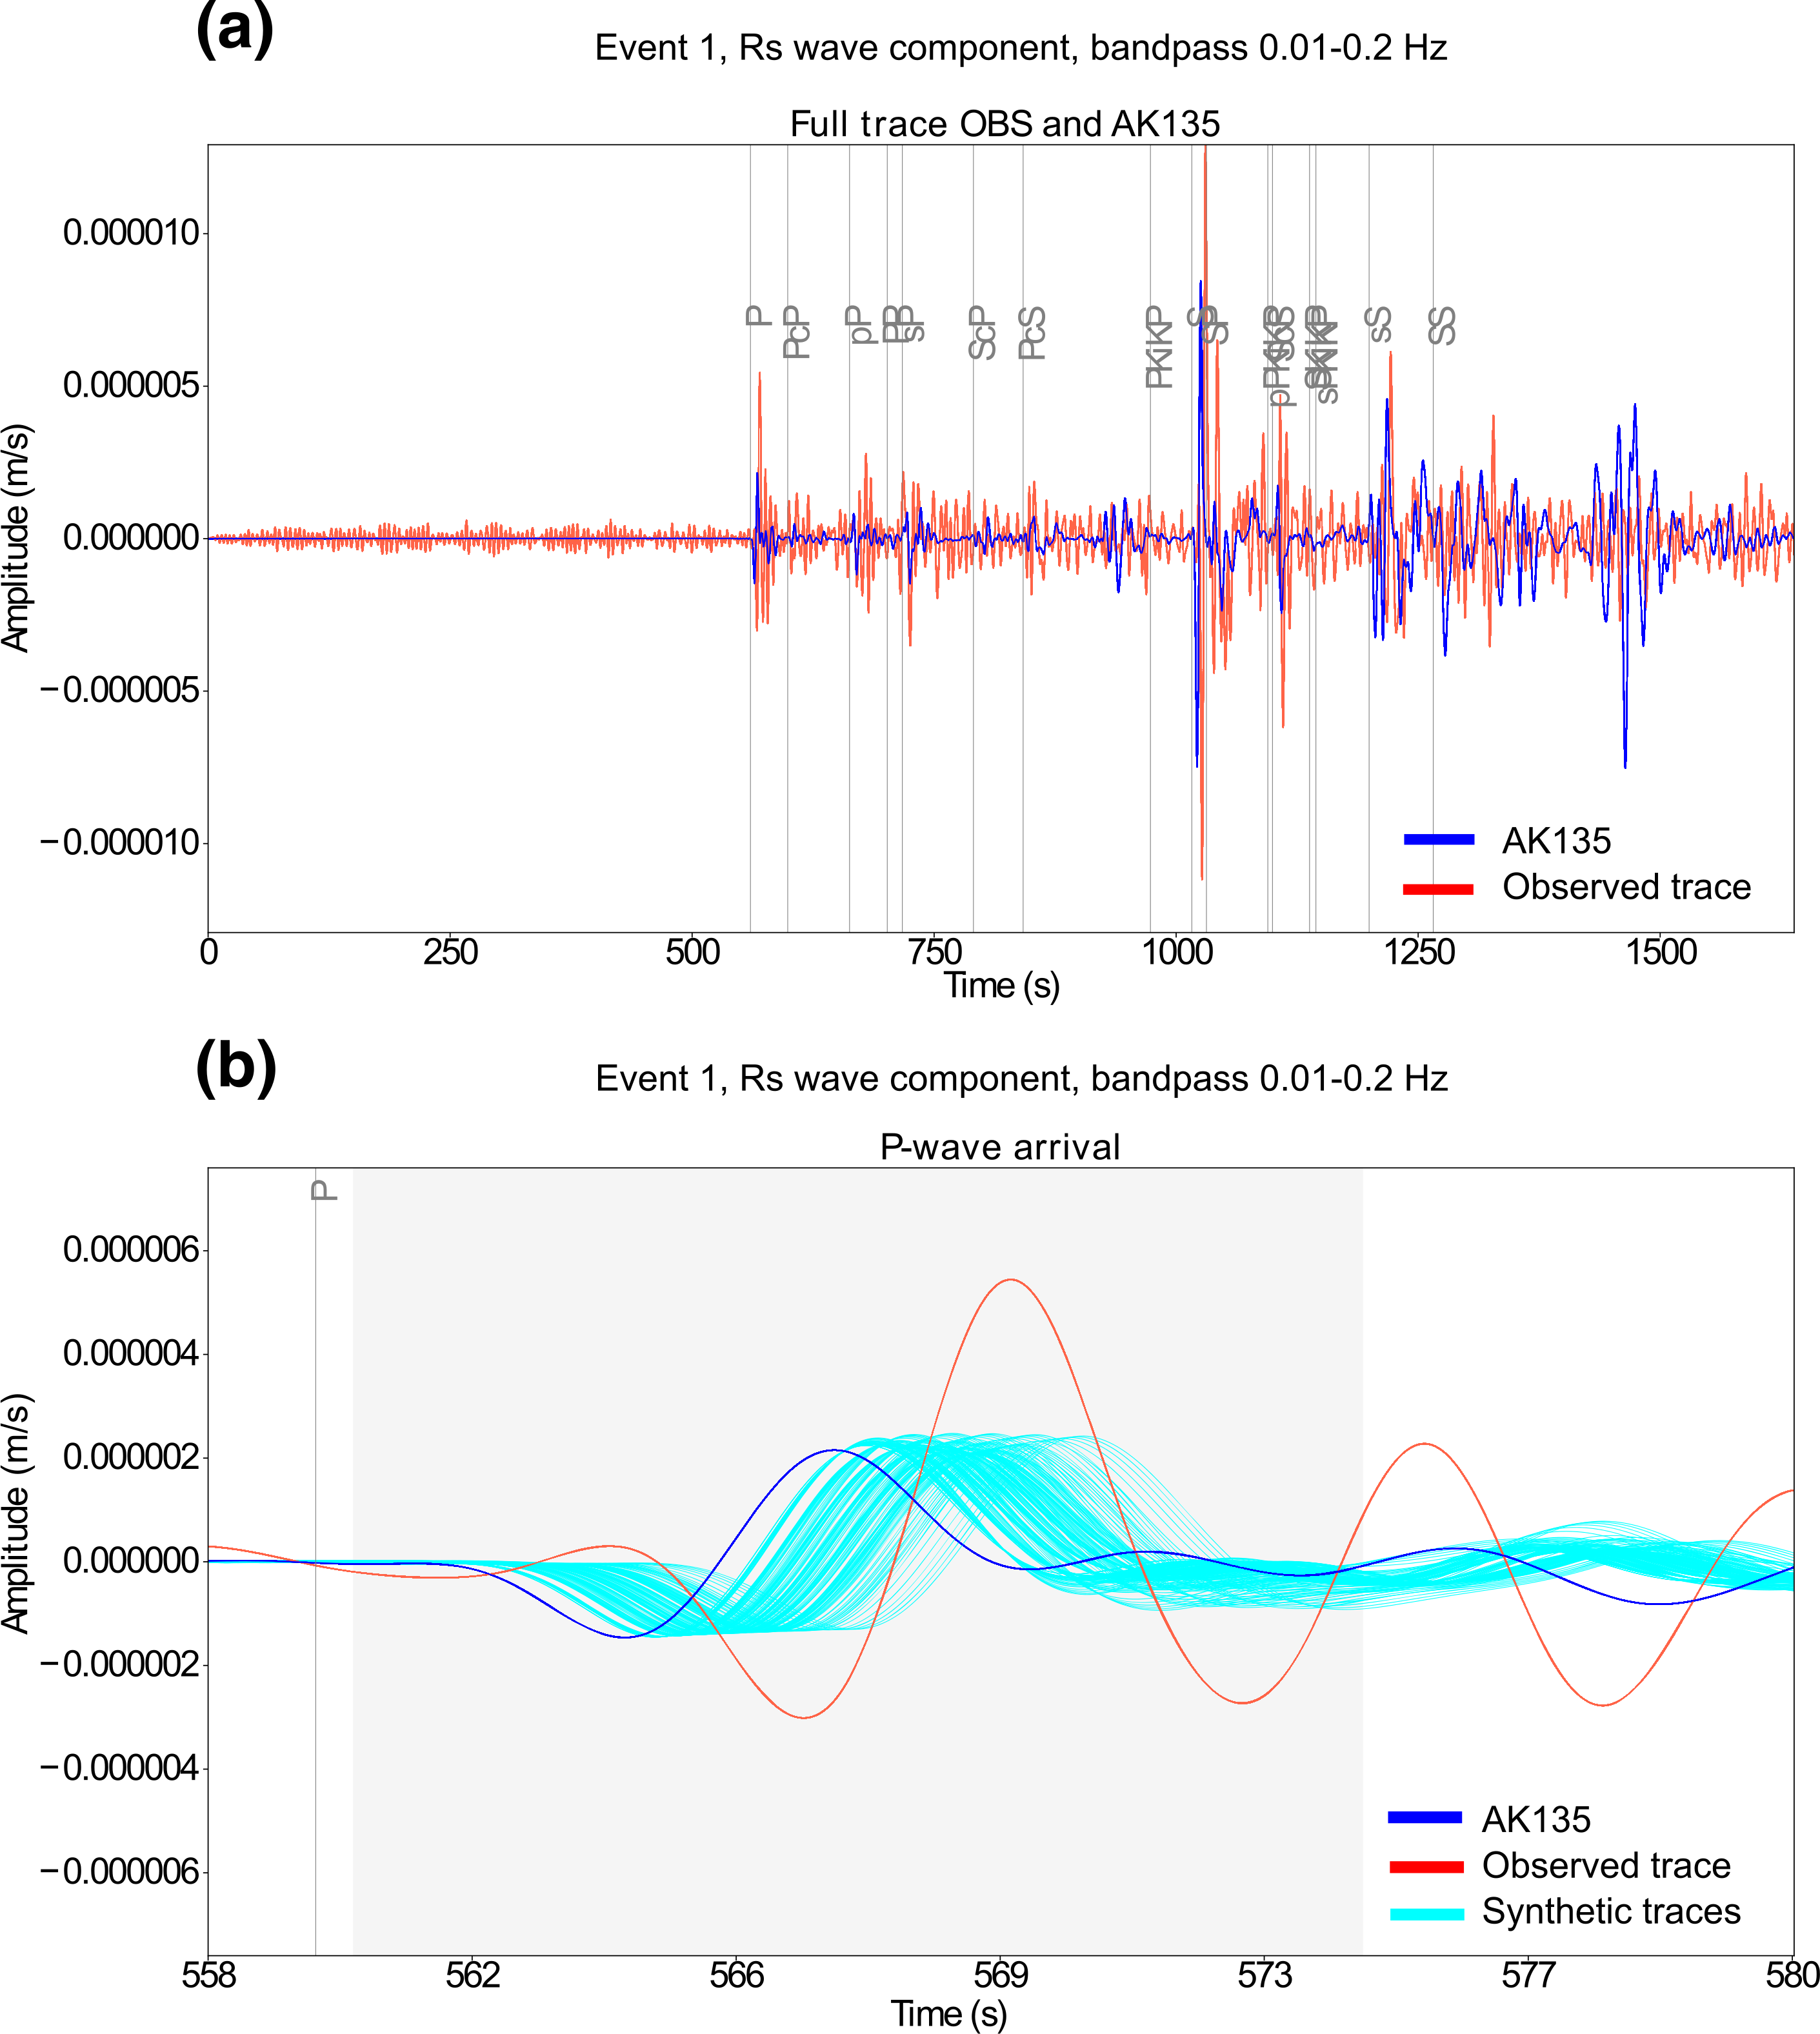
\includegraphics[width=8.6cm]{figures/ch2-franken1.png}
    \caption{Comparison of the observed and modelled seismic arrival at the RER Geoscope from the Bali Sea earthquake on the 10th March 2011 and with a source depth of 510\,km. (a) Seismogram containing the radial components of the full synthetic waveform generated for 1D Earth reference model ak135 (blue) and the observed seismic trace (red) for event 1, band-pass filtered from 0.01 to 0.2 Hz. (b) A close-up of the P-wave arrival of trace presented in (a), with the additional 210 synthetic traces (light blue) generated from a range of 1D melting models. The gray zone represents the automated cross-correlation window used to find the time shift with the observed trace. Figure is from \cite{franken-etal-2020}.}
    \label{fg:franken1}
\end{figure}

In the last four years I tried to push beyond the classic interpretation of inverse models that dominates Earth science and seismology in particular. Rather than creating methods to compare synthetic seismic structures with the inverted structures, I wanted to use the forward model to simulate the true observation: the seismic waveform recorded at the receiver (Figure \ref{fg:franken1}). In collaboration with Thijs Franken, Nobu Fuji, and Alexandre Fournier we focused on melt migration and how partial melt might impact seismic arrivals at La Réunion.  A strong low velocity region is imaged in tomographic models below La Réunion \citep{mazzullo-etal-2017}, and we could be tempted to assume it is due to high melt retention. However, by creating a 1D forward model of melt production and retention we can propagate numerically a seismic wave through this 1D system (Figure \ref{fg:franken1}). The arrival can then be compared to the observed waveforms, to try and find a best fit. This approach is more fully described in the PhD thesis of Thijs Franken and in \cite{franken-etal-2020}

\begin{figure}
    \centering
    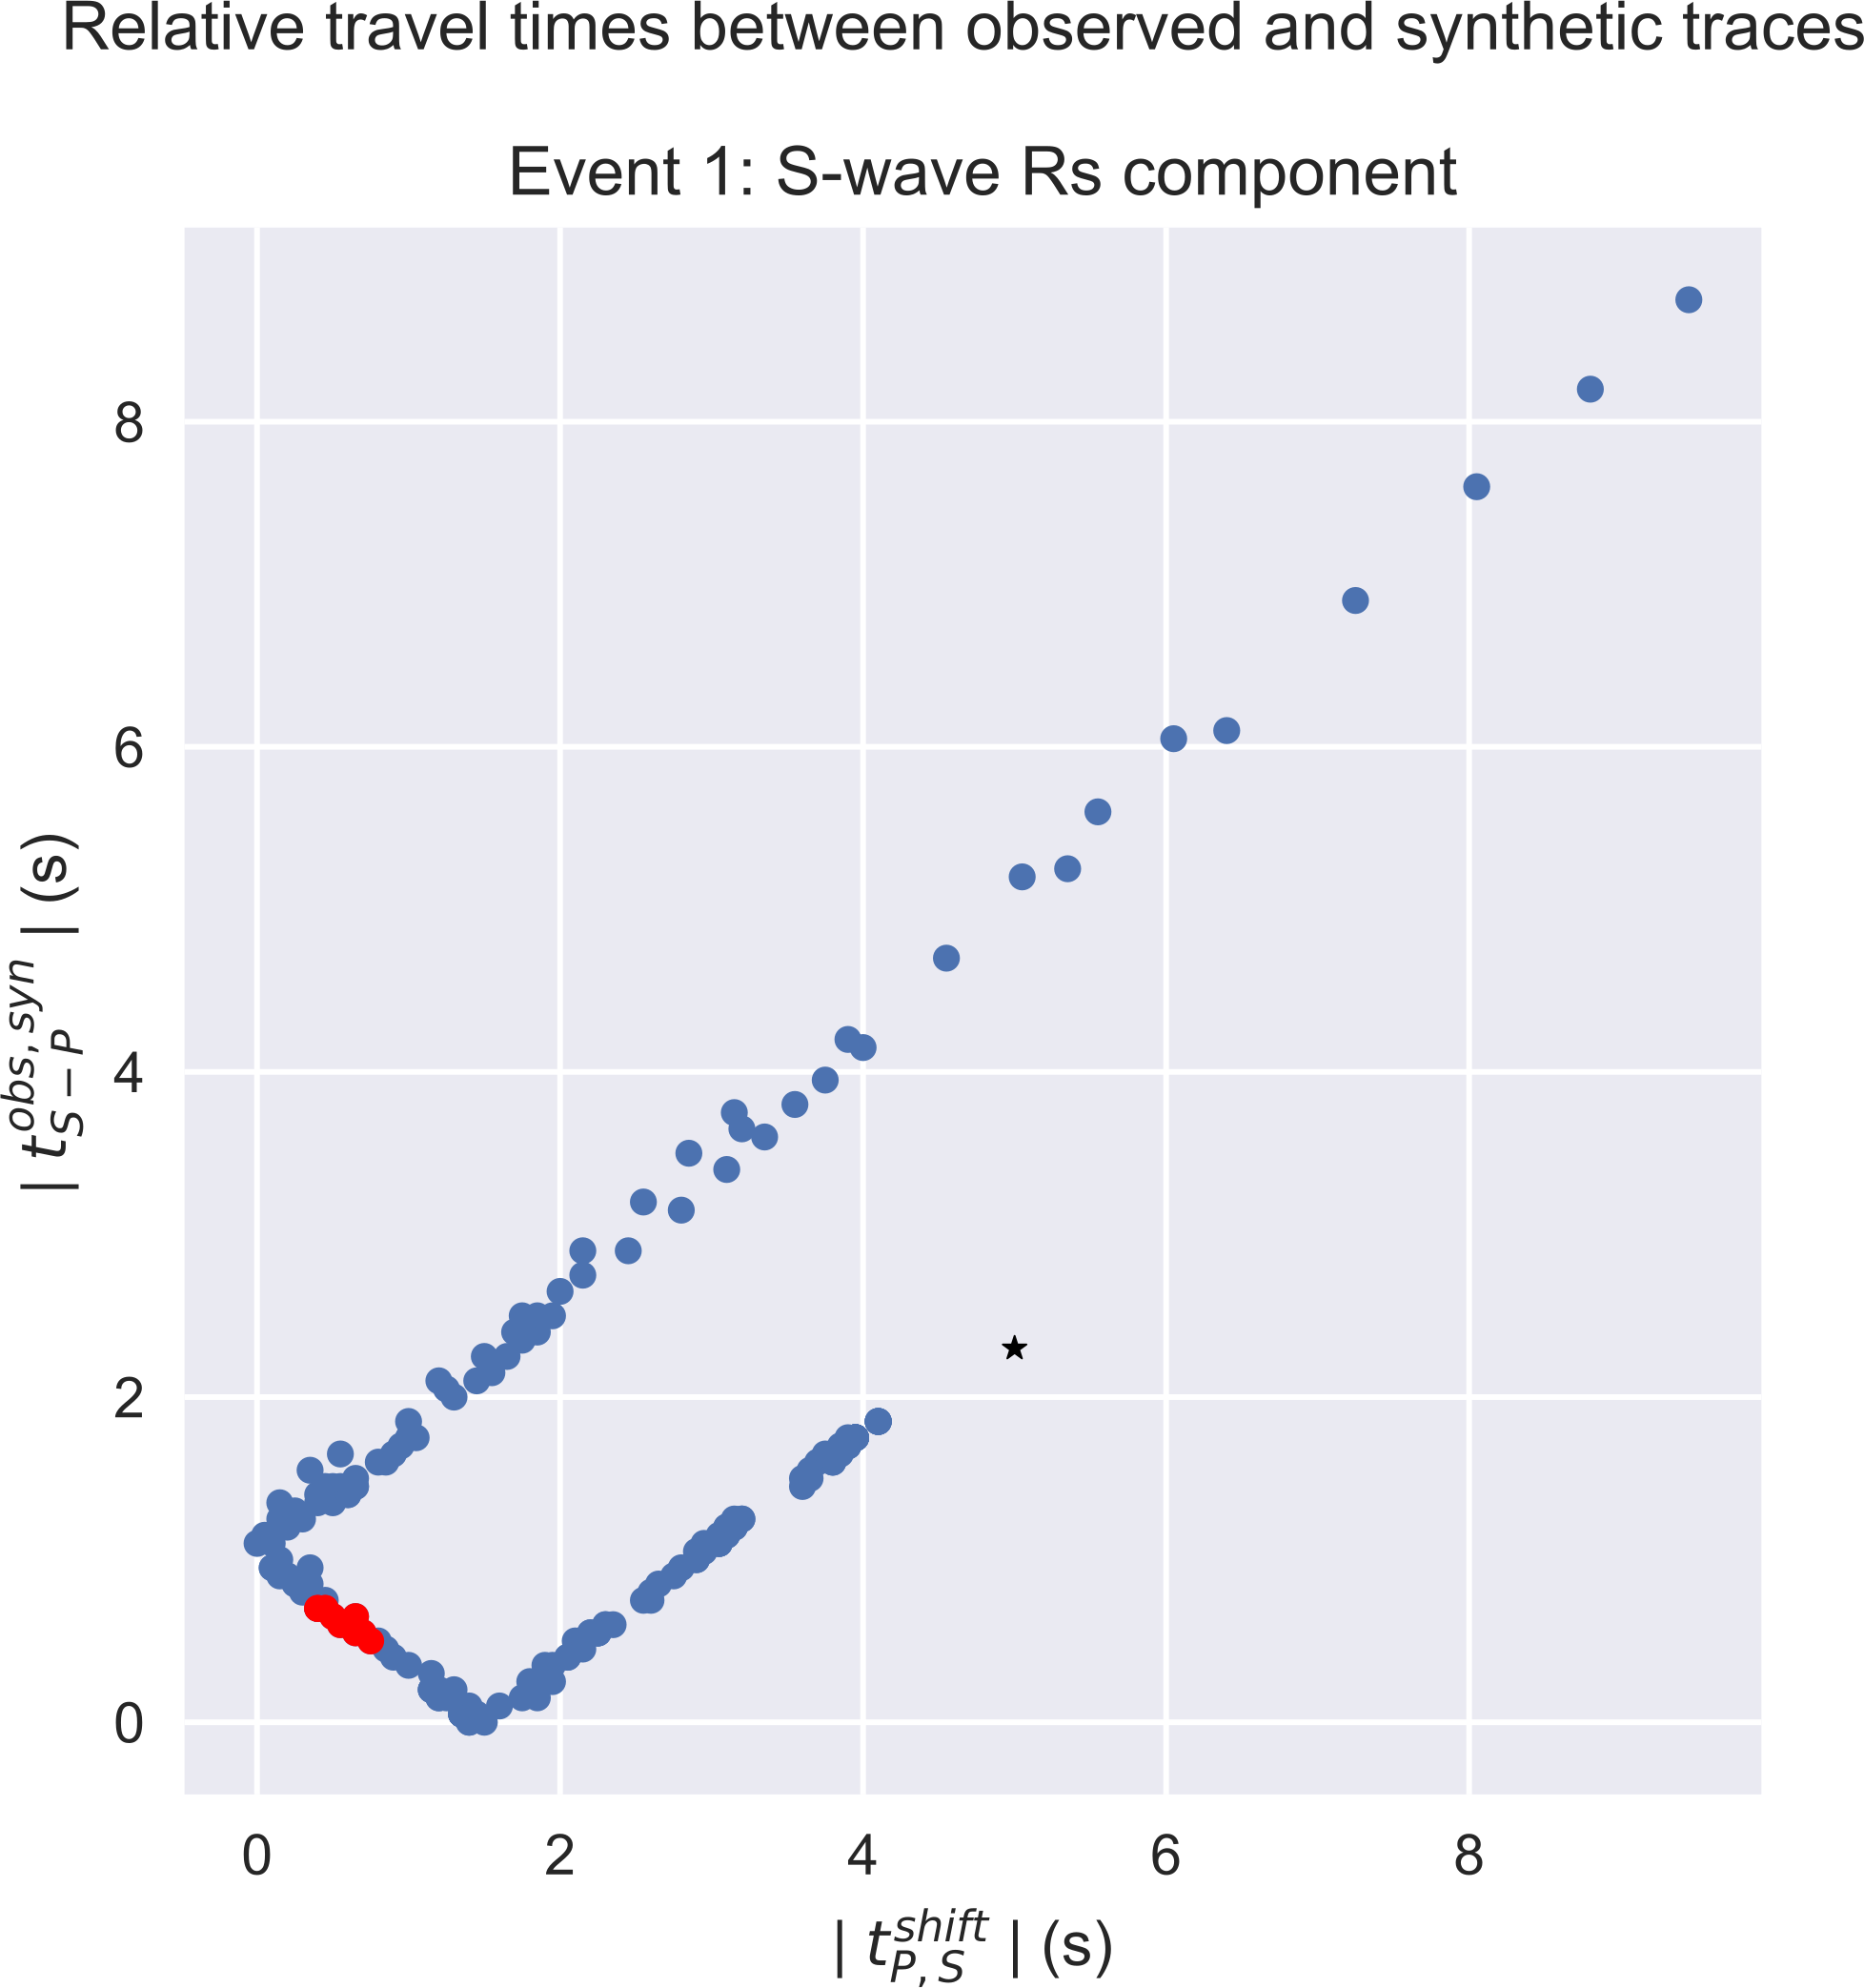
\includegraphics[width=8.6cm]{./figures/ch2-franken2.png}
    \caption{Absolute value of the travel time delay $| t^{shift}_{P,S} |$ versus the absolute value of the differential travel time $| t^{obs,syn}_{S-P} |$ for the radial component of the S-wave arrival from the Bali Sea earthquake (Figure \ref{fg:franken1}). Best-fit models by minimized RMS are displayed in red, whereas results for the 1D Earth reference model ak135 are presented by a black star. Figure is from \cite{franken-etal-2020}.}
    \label{fg:franken2}
\end{figure}


We ran models through the full parameter space for 1D melting and melt transport, and found that only a select few models could match the travel time difference and the S-to-P travel time differential when synthetic waveforms were compared to the observations at the RER Geoscope permanent station \citep{franken-etal-2020}. An example of the analysis is shown in Figure \ref{fg:franken2} for the Bali Sea earthquake shown in Figure \ref{fg:franken1}. We looked for the forward model of melt production and transport that would minimise the misfit between the travel time delay of the P- and S-arrival and the relative travel time difference between the P- and S-wave arrival. For the 21 earthquakes that had a sufficiently deep source and epicentral distance that gave teleseismic arrivals, the best fit models implied low melt retention and a hot mantle temperature ($\sim 1450\rm\,^{\circ}C$). This would suggest conditions below La Réunion of melt retention of $<$0.28\% and high melt extraction rates of 8.37-18.35 $\rm\,m\,yr^{-1}$ \citep{franken-etal-2020}, which would imply a melting system that can react rapidly, geologically speaking, to change. This is in line with the observations from Iceland \citep{armitage-etal-grl-2019}, and a more recent model where it was found that in order to match the observed change in volumes of melt erupted melt would have to travel at roughly $30\rm\,m\,yr^{-1}$ \citep{jones-2020}. The combined estimates of melt extraction rates from Iceland and La Réunion would therefore suggest that melt retention is low.

At the beginning of this chapter I introduced the hypothesis based on inverse seismic models that large quantities of melt are retained beneath regions of volcanism. This hypothesis is based in the interpretation that low seismic velocity anomalies can only be explained by lenses of melt reducing the speed at which seismic waves can travel. This hypothesis can be tested, and in doing so it is clear that melt is unlikely to be the cause of low velocity zones. Rather it is the combined effect of thermal attenuation and significantly smaller quantities of melt that create the travel time delays and changes in the observed waveforms \citep[e.g.][]{goes-etal-2012,armitage-etal-epsl-2015,armitage-etal-grl-2019,franken-etal-2020}. Hopefully in the future, seismological research will continue to move beyond the simple interpretation and start to test the hypothesis behind the interpretation (see for example \citealp{maguire-etal-2018}).

\section{Surface Processes}

The surface of the Earth contains the most time-sensitive record of the past. Accumulations of sediment can give information about change in climate, tectonics and even the mantle throughout geological time. However, as with the fields of seismology and geochemistry, the observations require interpretation to extrapolate how physical processes have impacted the geological record. As with melt generation and transport, sediments are created and transported to create the final observation: a stratigraphic section. Changes in the pattern of sediment deposition have for more than a century been interpreted for possible past forcing mechanisms. One of the most dominant paradigms is sequence stratigraphy. This is a set of rules where by stacking patterns of sedimentary deposits can be interpreted in terms of past change in sea-level, subsidence, and change in the sediment delivery to the zone of deposition \citep[e.g.][]{vail-etal-1977,vanwagoner-etal-1990,catuneanu-etal-2009}. Yet these rules are largely heuristic and are rarely tested.

Over the last decade I have developed numerical models to try and predict observations of grain size change in stratigraphic units (see Appendix \ref{app2}; \citealp{armitage-etal-ngeo-2011,armitage-etal-2015,armitage-etal-br-2018}). These numerical models reduce the level of complexity of the erosion and transport of material from the terrestrial source to eventual deposition in either alluvial fans or the shoreline. Despite their simplicity, they can be used to explore the implications of change in climate, sea-level, and subsidence within a sedimentary system. This means that interpretations based on observations can be tested. In this section I will describe two regions where I have developed numerical models to try and understand what caused the observed change sediment deposition: the Eocene Escanilla system in Spain and the Book Cliffs in central USA (the articles for these two examples are included within Annex B).

\subsection{Eocene Escanilla sedimentary system, Spain}

\begin{figure}
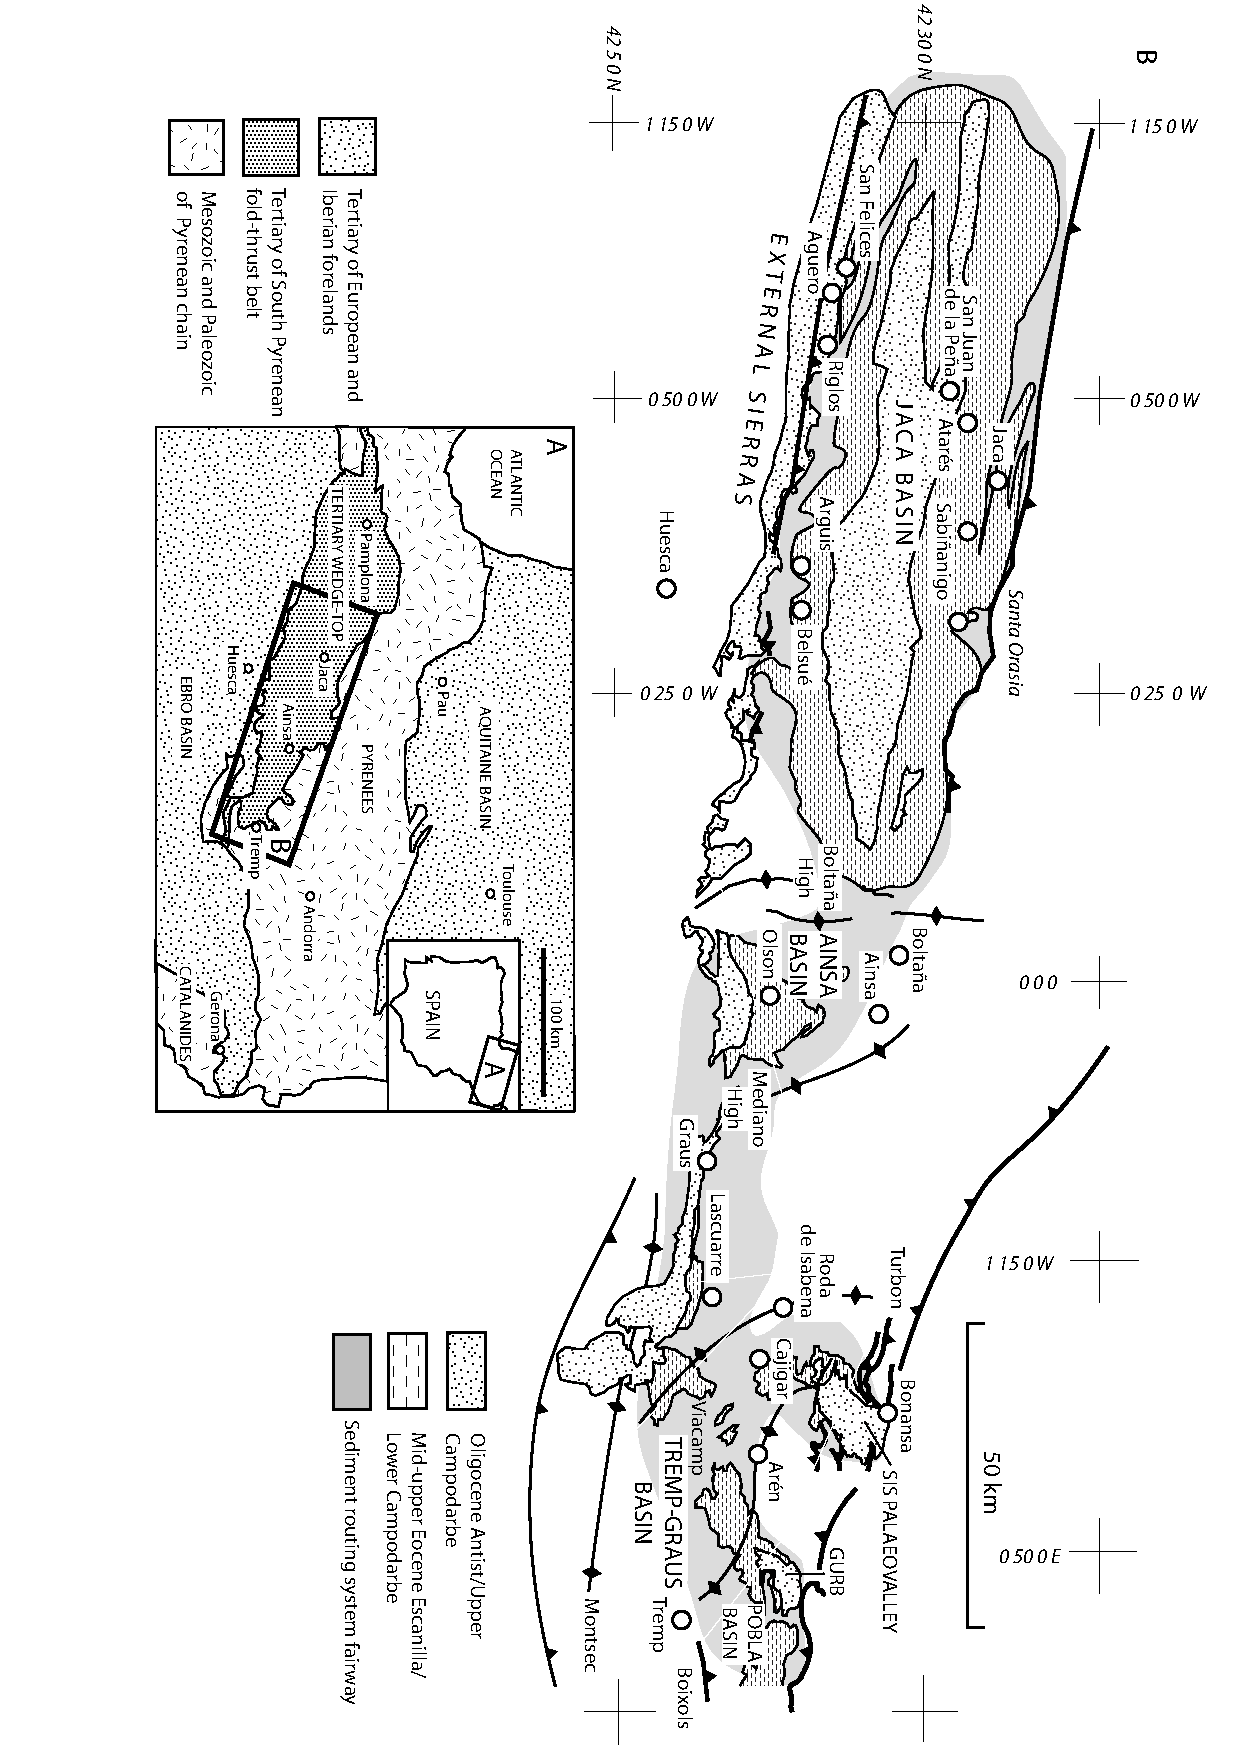
\includegraphics[height=\textwidth,angle=90]{./figures/ch2-escanilla-map.pdf}
\caption{A) Location of the Escanilla paleo--sediment-routing system in the Tertiary wedge top of the south-central Pyrenees, northern Spain. B) Detail of the Escanilla paleo--sediment-routing system fairway, after \cite{michael-etal-2014a}.}
\label{fg:escanilla-map}
\end{figure}

The Escanilla sediment-routing system has its source regions in the south-central Pyrnean orogen (Figure \ref{fg:escanilla-map}). Sediment was transported throughout the Lutetian to Priabonian (41.6 to 33.9\,Ma) from wedge top basins in the east to marine deposits in the west. It can be simplified into two major source regions that fed sediment into the Sis Paleaovalley and Pobla Basin (Figure\ref{fg:escanilla-map}). The sediment fairway can then be simplified to a single depositional cross section that extends from the Gurb-Pobla and Sis depocenters through the Tremp-Graus, Ainsa, and Jaca basins (Figure \ref{fg:escanilla-map}; \citealp{michael-etal-2013}). The position of the limit of gravel deposition, the gravel front, and sand deposition, the sand front, for three time periods were measured by Nicolas Michael and Philip Allen \citep{michael-etal-2013}. It was found that the gravel front migrated westwards significantly in the final time period, from 36.5 to 33.9\,Ma. A classic interpretation of this progradation would be that there was increased precipitation within this third time period, which lead to increased energy within the system and the migration of the gravel front towards the west.

\begin{figure}
\centering
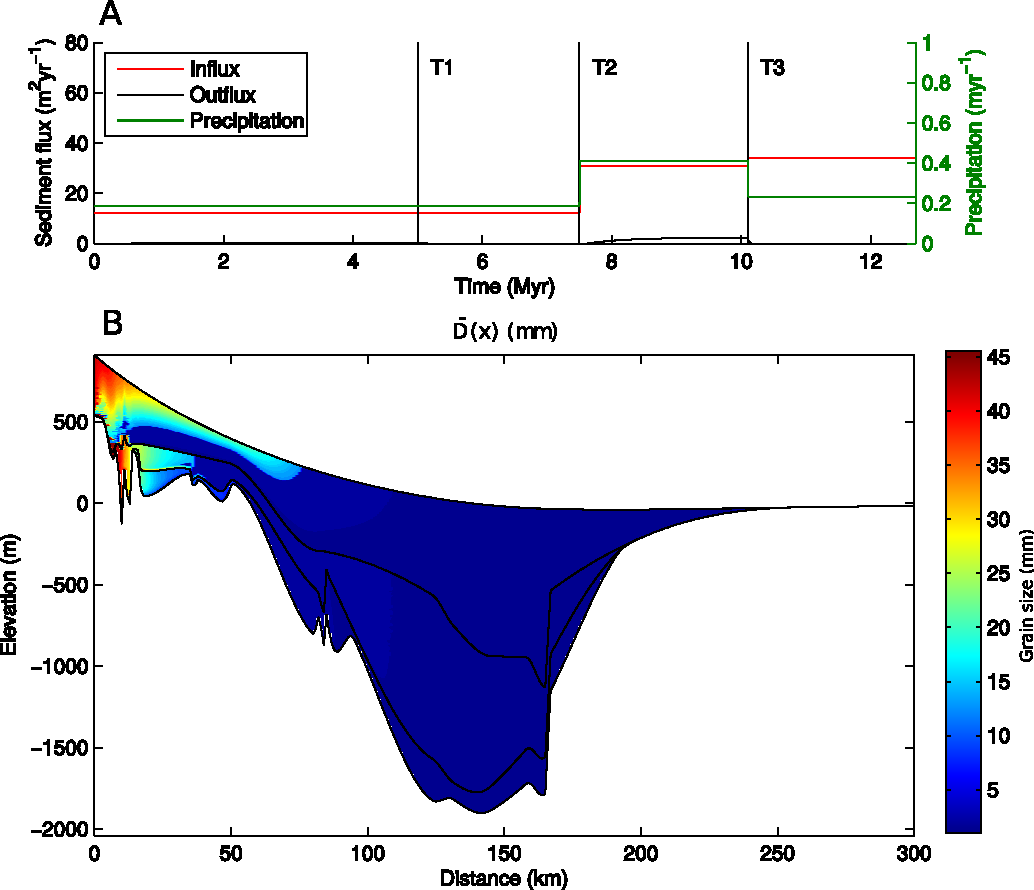
\includegraphics[width=8.6cm]{./figures/ch2-escanilla-model.pdf}
\caption{Stratigraphic architecture predicted by the forward model run that most closely matches the observed location of the gravel front. A) Sediment flux in and out of the basin and precipitation rate against time. B) Distribution of grain-size deposited in the idealized Escanilla paleo--sediment-routing system.}
\label{fg:escanilla-model}
\end{figure}

The potential causes of the observed progradation can be explored using forward models of sediment transport. By using a 1D model for sediment transport that I developed \citep{armitage-etal-ngeo-2011}, Monte-Carlo--like simulations were run to find the combination of change in surface run-off and catchment erosion that could match the position of the gravel and sand fronts within the system \citep{armitage-etal-2015}. The best fitting model suggests that precipitation increased significantly in the middle time period, and not the third time period (Figure \ref{fg:escanilla-model}). The reason the gravel front did not migrate with this change in precipitation is because input sediment flux rose to fill the extra accommodation space created. It was not until time period three where precipitation rates fell despite similar sediment flux input, that there was significant progradation of gravel towards the coastline. For a more detailed explanation see the full article in the Annex B.

\subsection{Book Cliffs, USA}

\begin{figure}
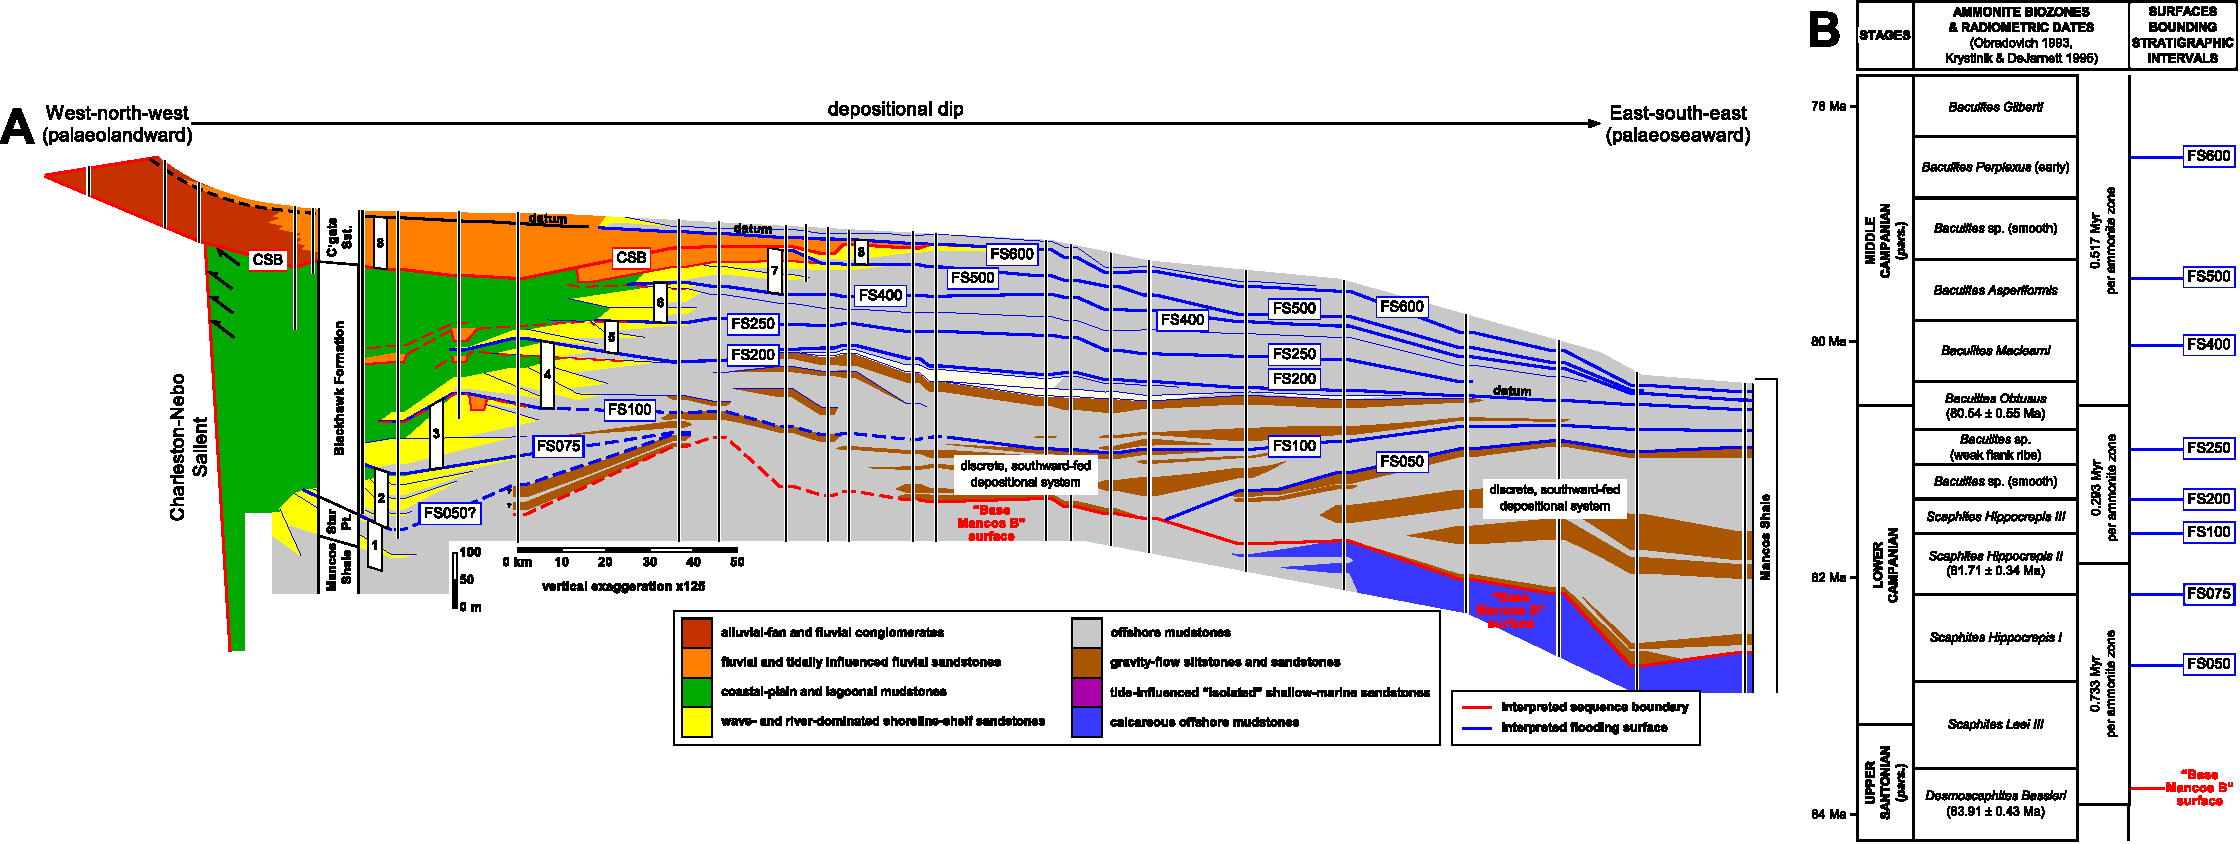
\includegraphics[width=\textwidth]{./figures/ch2-bookcliffs.pdf}
\caption{(a) Correlation panel illustrating stratigraphic architecture through the Book Cliffs outcrops and adjacent areas (after \citealp{horton-etal-2004,hampson-2010,hampson-etal-2014}; and references therein). Interpreted major flooding surfaces and erosional unconformities (sequence boundaries) are labelled. Deposits corresponding to time intervals 1--8 are indicated. Up system correlation of the lower part of the Castlegate Sandstone (time interval 8) is after \cite{robinson-1998} and \cite{mclaurin-2000}. A variety of stratigraphic surfaces are used as datum surfaces for different parts of the panel, and each surface is assigned the depositional dip of an eastward-dipping coastal plain or shelf profile where used as a datum. (b) Ammonite biostratigraphy, radiometric dates \citep{obradovich-1993}, and estimated ammonite biozone durations \citep{krystinik-1995} for the studied strata, showing the interpreted ages of major flooding.}
\label{fg:bookcliffs}
\end{figure}

The Book Cliffs of eastern Utah and western Colorado, USA, expose a record of a large palaeo-sediment-routing system. This is a classic site, where ancient clonglomeratic alluvial deposits transform into shoreline sandstones, marine deposits and shales (Figure \ref{fg:bookcliffs}). In collaboration with Philip Allen, Peter Burgess, and Gary Hampsen, we decided to explore if the migration of the gravel front, sand front, and shoreline within this sedimentary system could likewise be `inverted' for past forcing. The classic interpretation has been that cyclic progradation and retrogradation of the shoreline and sand front is due to cyclic sea level change (this is the birth place of sequence stratigraphy). The sediment transport equation (equation \ref{eq:transport}) was modified to include a transport law that was active when the surface was below sea level \citep{kaufman-etal-1991,armitage-etal-br-2018}. This heuristic model approximates the effect of tidal energy on moving sediment away from the shoreline. With this addition the effect of change in sea-level and surface run-off could be explored \footnote{This model has most recently been added to a 2D visco-elasto-plastic model of lithosphere and crustal extension to explore sedimentary patterns during continental extension, see \cite{perez-gussinye-etal-2020}}.

\begin{figure}
\centering
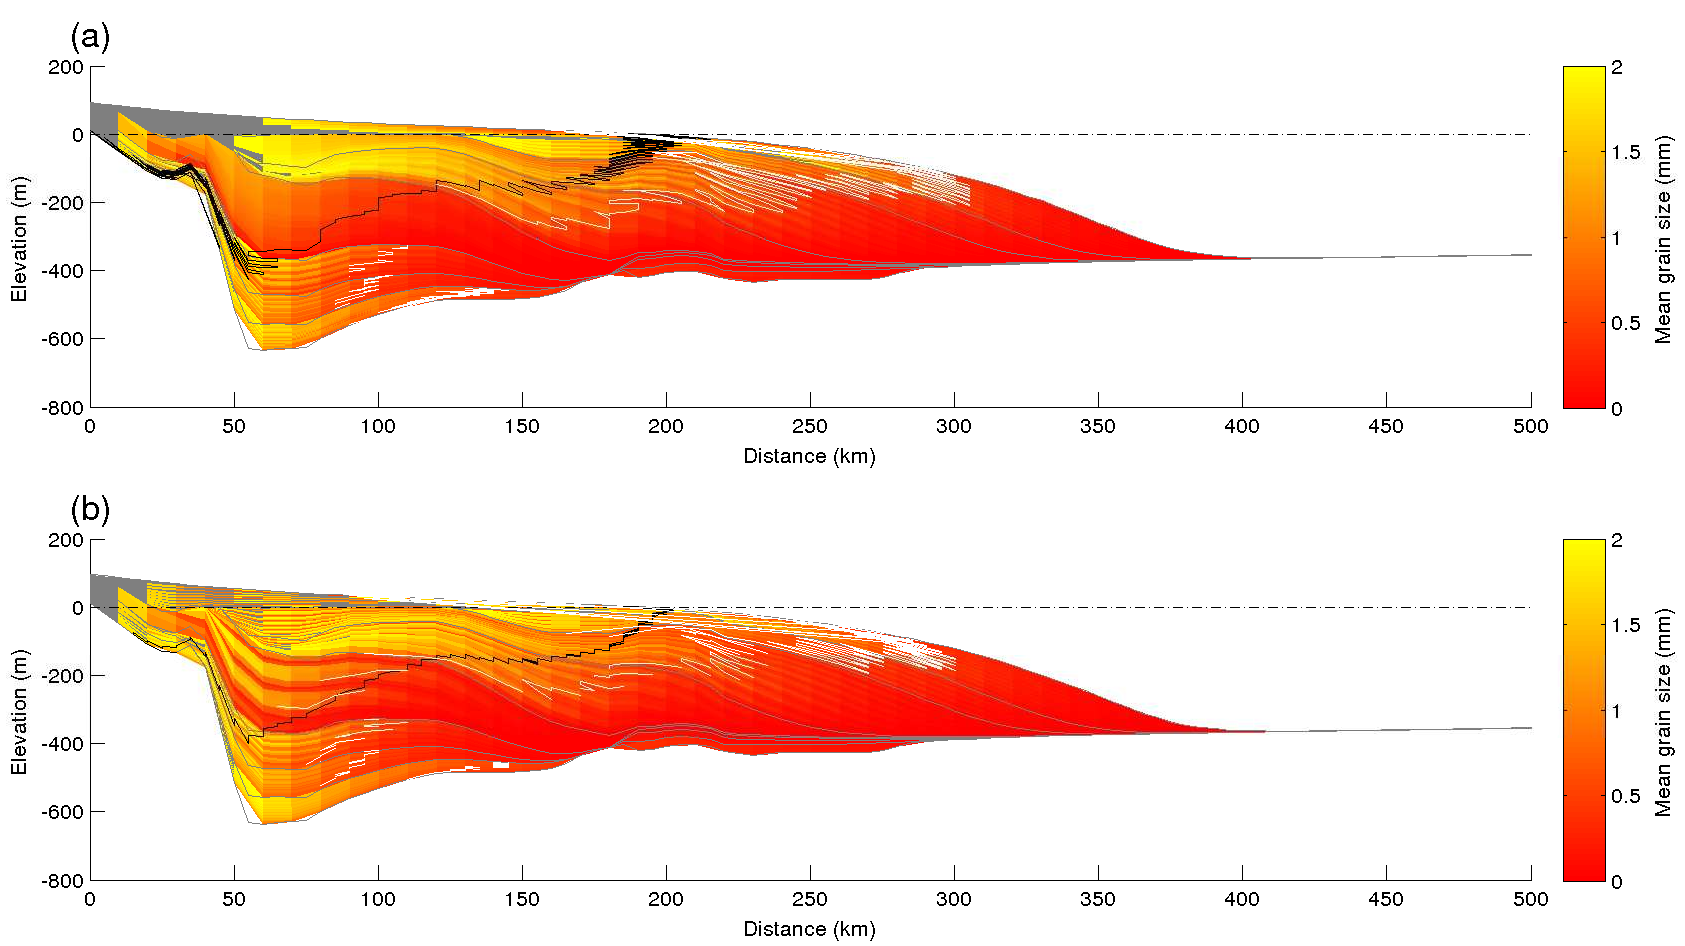
\includegraphics[width=10cm]{./figures/ch2-bookcliffs-model.pdf}
\caption{Synthetic strata for two models of the stratigraphic architecture in the Star Point -- Blackhawk -- lower Castlegate wedge, based on the Book Cliffs outcrops. (a) Predicted stratigraphic architecture assuming a 100\,kyr periodic oscillation in relative sea-level of amplitude $\pm 10\rm\,m$. (b) Predicted stratigraphic architecture assuming a 100\,kyr periodic oscillation in precipitation rate of amplitude $\pm 50$\,\%. Regions of gravel grains are blocked out in grey. The mean grain size of grains finer than 2\,mm in diameter is plotted. The shoreline position through time is marked as a solid black line, and the dashed black line marks sea level.}
\label{fg:bookcliffs-model}
\end{figure}

When the sediment transport model was applied to the Book Cliffs outcrop data the results showed that both high frequency (period of 100\,kyr) sea level change and change in surface run-off can impact the sand front and shoreline (Figure \ref{fg:bookcliffs-model}). However, change in terrestrial forcing also impacted the gravel front. If we assume that the observed depositional thickness of sediment is representative of the sediment flux into the basin, then the migration history of the gravel front would be a quantifiable measure to distinguish whether cyclical patterns of progradation and retrogradation were the result of cyclical change in precipitation rates or sea level (Figure \ref{fg:bookcliffs-model}). Data describing the architecture of proximal deposits in the Star Point -- Blackhawk -- lower Castlegate -- Mancos sediment-routing system are rare, however, on balance the evidence suggests limited movement of the gravel front. Therefore, a high-frequency cyclical change in relative sea level is the most probable of modelled mechanisms to account for the observed stratigraphic architecture. For a more detailed explanation see the full article in the Annex B.

This study, and the previous example from the Escanilla system, demonstrate the potential of applying physical models to test hypothesis (or interpretations) drawn from sedimentological observations. In both cases, the models gave insights into how the sedimentary system might respond to change, and how signals are transformed down system \citep{armitage-etal-ngeo-2011}. This style of model is currently being used to investigate late-Pleistocene to Holocene deposition in alluvial fans within Death Valley \citep[see][]{brooke-etal-2018}. Sam Brooke has advanced upon the transport model by adding infiltration, methods to account for storm variation, and a more physically based grain-size sorting. Early results would suggest that an increase in the frequency of storms will have just as a significant effect on the gravel front as an increase in mean run-off. 

\section{Predicting geological observations}

In Earth science the observations can become confused with interpretations. A tomographic image of the Earth's interior is not an observation, it is the result of an inversion and is therefore subject to various artefacts due to regularisation and the quality of the input data. Stratigraphic sections are images created by interpolating sparse observations of rock type and age, from which an image is created that gives a sense of the distribution of sedimentary deposits. A stratigraphic section, like a tomographic image, is not an observation. Yet, it is tempting to treat these models as observations.

The core of my research has been to try and use numerical models to predict observations. This has evolved from predicting crustal velocities, major element oxides, and rare Earth compositions in basaltic glass during my post PhD research \citep{armitage-etal-2010,armitage-etal-g3-2011}, to predicting grain size within sedimentary deposits in sedimentary basins \citep[e.g.][]{armitage-etal-ngeo-2011,armitage-etal-2015,armitage-etal-br-2018}, fan topography on Mars \citep{armitage-etal-grl-2011}, basin subsidence in various locations \citep[e.g.][]{armitage-2010,armitage-etal-jgr-2013,petersen-etal-2015}, upper mantle seismic tomography at various locations \citep[e.g.][]{goes-etal-2012,armitage-etal-2015}, and more. One of the biggest challenges has been breaking down the seismic inverse models and getting to the actual observation, the seismic waveform.

In a large collaborative effort with David Ferguson, Saskia Goes, James Hammond, Eric Calais, Kate Rychert and Nick Harmon, we tried to use both observations from igneous geochemistry and inverse models from seismic stations, to understand the structure of the upper mantle below Afar \citep{armitage-etal-epsl-2015}. Here I found that the forward geodynamic model could consistently predict the lava chemistry and seismic tomography from surface waves. However, it could not predict the seismic velocity structure required from the inversion of S-to-P receiver functions. From this failure I decided to build a research project where the seismic observation, the displacement recorded at the seismometer, would be predicted. This involved a new collaboration with Nobu Fuji, Alexandre Fournier, and our PhD student Thijs Franken. The result is a new scientific work-flow where the forward geodynamic model is transformed in to a seismic structure. This structure is used as an input for forward wave propagation, and the subsequent seismic arrival is compared with the arrival at the earth's surface \citep{franken-etal-2020}. I am convinced that this is the direction in which Earth science should go.

\begin{subappendices}

\section{A simplified model of decompression melting}\label{app1}

\begin{figure}
\centering
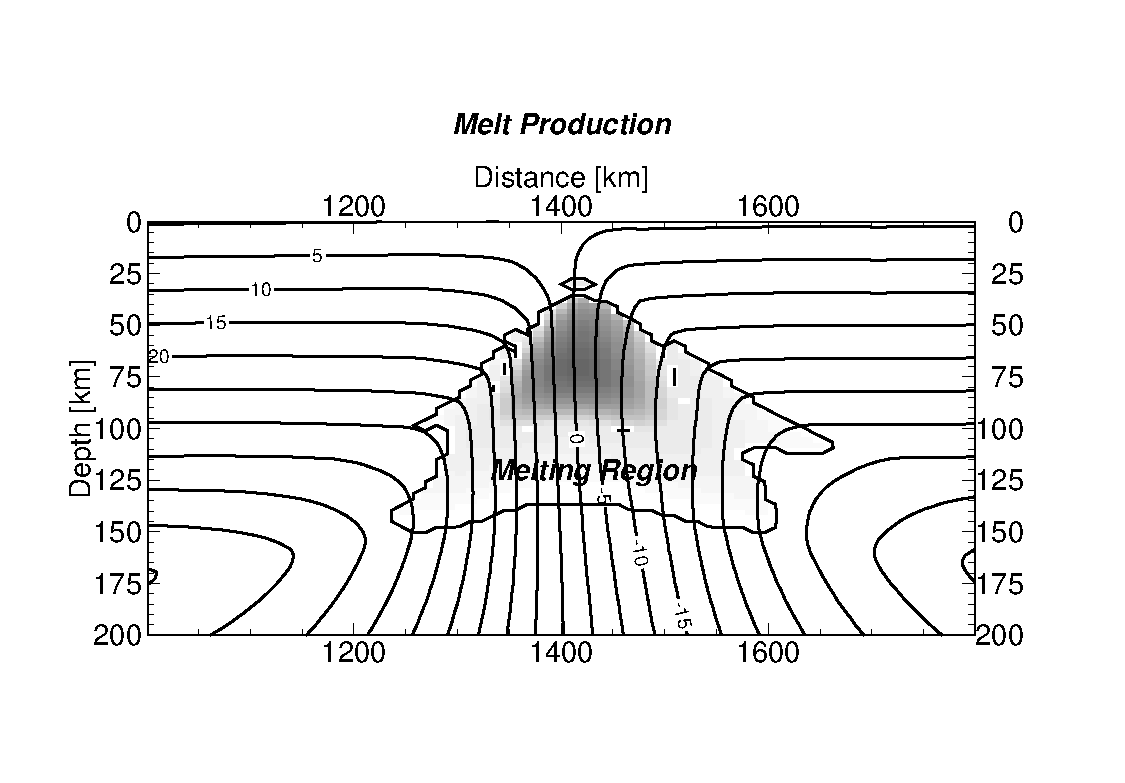
\includegraphics[width=8.6cm]{./figures/ch2-melt-region.pdf}
\caption{Diagram of the zone of partial melting with stream lines of mantle flow.}
\label{fg:melt-region}
\end{figure}

Decompression melting occurs when the mantle loses pressure due to vertical movement and the rock matrix crosses the solidus (Figure \ref{fg:melt-region}). To numerically model this process we need a set of continuum equations, which in this case are Stokes equations, the conservation of momentum and mass, and the conservation of energy. The conservation of momentum is,
\begin{equation}
\nabla \cdot \sigma + f = 0,
\end{equation}
where $\sigma$ is stress, the sum of the viscous stresses and pressure, and $f$ is the applied force, which in this case is due to gravity, $\Delta\rho g$. It is typical in geodynamics to then seperate out the viscous and pressure terms,
\begin{equation}
- \nabla \cdot \tau + \nabla p + \Delta\rho g \hat{\mathbf{z}} = 0,
\label{eq:momentum}
\end{equation}
where $\tau$ is the deviatoric stress, $p$ is pressure, $\Delta\rho$ is the density change due to thermal and chemical change (melting), $g$ is the acceleration due to gravity, and $\hat{\mathbf{z}}$ is a unit vector in the vertical direction.

The conservation of energy can be expressed as \citep[e.g.][]{ribe-1985},
\begin{equation}
\frac{\partial T}{\partial t} + \bar{\mathbf{v}} \cdot \nabla T - \kappa\nabla^{2} T + mL = 0,
\label{eq:energy}
\end{equation}
where $T$ is temperature, $\bar{\mathbf{v}}$ is the average velocity of the solid mantle and melt, $\kappa$ is the thermal diffusion coefficient, $m$ is the melt production rate, and $L$ is the latent heat of fusion. The latent heat is given by $L = T\Delta S/C_{p}$, where $\Delta S$ is the entropy change due to melting and $C_{p}$ is the heat capacity. The average velocity is given by \citep{scott-1992},
\begin{equation}
\bar{\mathbf{v}} = \left(1-\phi\right)\mathbf{v}_{s} + \phi \mathbf{v}_{l},
\label{eq:average-velocity}
\end{equation}
where $\phi$ is porosity, $\mathbf{v}_{s}$ is the solid mantle velocity, and $\mathbf{v}_{l}$ is the melt velocity. The conservation of mass is given by,
\begin{equation}
\frac{\partial \rho}{\partial t} + \nabla \cdot \left(\rho \bar{\mathbf{v}} \right) = 0.
\end{equation}
I take the simpligying assumption that density for the solid and liquid phase are the same, except for within the momentum balance, the \emph{Bousinesq approximation}. This means that the mass balance becomes,
\begin{equation}
\nabla \cdot \bar{\mathbf{v}} = 0
\label{eq:mass}
\end{equation}
In the case where there the melt phase is not explicitly modelled, the three equations can be solved various numerical methods such as finite difference \citep[e.g.][]{armitage-etal-g3-2018}, finite element \citep[e.g.][]{armitage-etal-2008}, or finite volume \citep[e.g.][]{civiero-etal-2019}.

If melt is to be included then the conservation of the liquid phase is written as,
\begin{equation}
\partial
\frac{\partial \phi}{\partial t} + \nabla \cdot \left( \phi \mathbf{v}_{l} \right) = m.
\label{eq:mass-melt}
\end{equation}
In this case to create a closed set of equations we need to relate the solid mantle velocity to the liquid melt velocity. If we assume that the melt percolates through a porous medium we can assume that the flows can be related by Darcy's law,
\begin{equation}
\phi\left( \mathbf{v}_{l}-\mathbf{v}_{s} \right) = \frac{k_{0}\phi^{n}}{\eta_{l}}\left( \Delta\rho_{m}g\hat{\mathbf{z}} + \nabla P \right),
\label{eq:darcy}
\end{equation}
where $k_{0}$ is the permeability coefficient (not well constrained), $n$ is the exponent on the assumed power relation between permeability and porosity, $\Delta\rho_{m}$ is the density difference between melt and the solid mantle, and $P$ is the pore pressure. I will simplify equation \ref{eq:darcy} by assuming that the compaction length scale is small, the `zero-compaction length approximation' \citep{ribe-1985}. This means that Darcy's law becomes,
\begin{equation}
\phi\left( \mathbf{v}_{l}-\mathbf{v}_{s} \right) = \frac{k_{0}\phi^{n}}{\eta_{l}}\Delta\rho_{m}g\hat{\mathbf{z}},
\end{equation}
and by substituting for the average velocity (equation \ref{eq:average-velocity}) we get and considering the veritcal flow only,
\begin{equation}
v_{l}-\bar{v} = \frac{k_{0}\phi^{n-1}}{\eta_{l}}\Delta\rho_{m}g.
\end{equation}
This allows the substitution for $v_{l}$ within equation \ref{eq:mass-melt}. However there remains one fundamental unknown, and that is the relationship between permeability and porosity. The value of $n$ in equation \ref{eq:darcy} is estimated to between 2 and 3. The most recent laboratory experiments would suggest that for mantle rock $n = 2.6\pm0.2$ \citep{miller-etal-2014}. Mathematically it is more expedient to assume that $n$ is an integer, therefore it has been assumed to be either 2 \citep[e.g.][]{scott-1989,goes-etal-2012} or 3 \citep[e.g.][]{hewitt-2010,armitage-etal-grl-2019}. Assuming $n=3$ the conservation of melt can be written as,
\begin{equation}
\frac{\partial \phi}{\partial t} + \bar{v}\frac{\partial \phi}{\partial z} + \frac{3k_{0}\Delta\rho_{m}g}{\eta_{l}}\phi^{2}\left( 1-\frac{4}{3}\phi \right)\frac{\partial \phi}{\partial z} = m.
\end{equation}
This non-linear 1D partial differential can be solved numerically using various iterative techniques \citep[e.g.][]{armitage-etal-grl-2019,franken-etal-2020}.

\begin{figure}
\centering
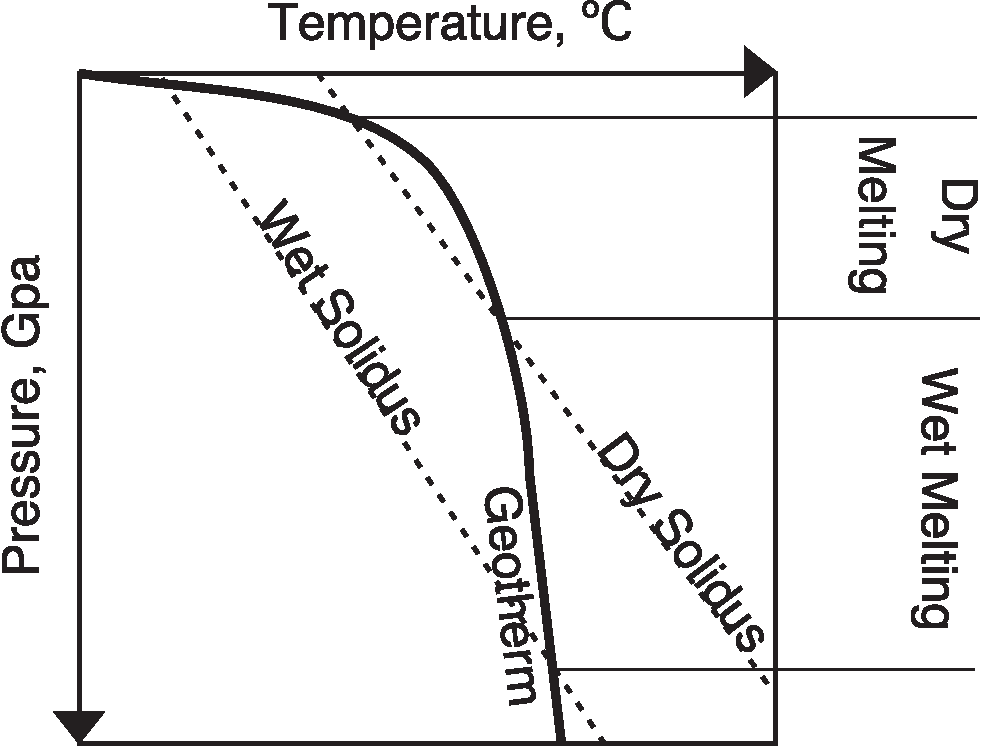
\includegraphics[width=8.6cm]{./figures/ch2-solidi-geotherm.pdf}
\caption{Diagram of the mantle geotherm crossing the wet and dry solidus.}
\label{fg:solidus}
\end{figure}

The conservation of energy and mass are coupled by the melt production rate, which is calculated from the temperature difference above the solidus. This solidus is a function of volatile content, depletion, temperature, and pressure (Figure \ref{fg:solidus}). In the energy balance I ignore the loss of heat due to decompression, but the adiabatic gradient needs to be accounted for within the thermodynamic balance for the melting equations. Assuming the mantle is dehydrated, no volatiles, it is calculated as,
\begin{equation}
T_{Sdry} = T_{S0} + \frac{\partial T_{S}}{\partial F}\vert_{p}F + \left(\frac{\partial T_{S}}{\partial p}\vert_{F} + \frac{\alpha T_{0}}{\rho C_{p}}\right)p,
\label{eq:dry-solidus}
\end{equation}
where $\partial T_{S}/\partial F\vert_{p}$ is the solidus depletion gradient, $F$ is depletion, $\partial T_{S}/\partial P\vert_{F}$ is the solidus pressure gradient, $\alpha$ is the coefficient of thermal expansion, $T_{0}$ is the mantle potential temperature, $C_{p}$ is the heat capacity, and $p$ is pressure. The solidus is assumed to deepen in the presence of water,
\begin{equation}
T_{Swet} = T_{Sdry} + K\left(D_{H_{2}O}C_{H_{2}O}\right)^{\gamma},
\label{eq:wet-solidus}
\end{equation}
where the coefficients $K$ and $\gamma$ are from the parametrisation of \cite{katz-etal-2003}, $D_{H_{2}O}$ is the partition coefficient for water, and $C_{H_{2}O}$ is the concentration of water within the solid mantle. Therefore the melt productivity is given by,
\begin{equation}
m = \frac{\Delta T}{L + \frac{\partial T_{S}}{\partial F}\vert_{P} + \frac{\partial T_{S}}{\partial F}\vert_{H_{2}O}},
\label{eq:melt-productivity}
\end{equation}
where $\Delta T = T-T_{S}$ is the temperature difference between the mantle and the solidus, and $\partial T_{S}/\partial F\vert_{H_{2}O}$ is the solidus depletion gradient during the melting of a hydrated mantle. This is calculated using the chain rule,
\begin{equation}
\frac{\partial T_{S}}{\partial F}\vert_{H_{2}O} = \frac{\partial T_{S}}{\partial C_{H_{2}O}} \frac{\partial C_{H_{2}O}}{\partial F}.
\end{equation}
The change in water composition as a function of depletion is calculated  assuming a mass balance between the partitioning of water between the solid and melt phase,
\begin{equation}
\frac{\partial C_{H_{2}O}}{\partial F} = -C_{H_{2}O} \frac{1}{D_{H_{2}O}}\left(1-F\right)^{\frac{1}{D_{H_{2}O}}-2}
\end{equation}
and the gradient in solidus with water composition is from equation \ref{eq:wet-solidus},
\begin{equation}
\frac{\partial T_{S}}{\partial C_{H_{2}O}} = \gamma K\left(D_{H_{2}O}C_{H_{2}O}\right)^{\gamma-1}
\end{equation}

To track the composition of the melt I assume disequilibrium melting, where the conservation of the solid composition, $C_{s}$, is given as \citep{spiegelman-1996},
\begin{equation}
\frac{\partial C_{s}}{\partial t} + v_{s}\frac{\partial C_{s}}{\partial z} = \left(\frac{1}{D} - 1\right) \frac{C_{s}m}{1-\phi},
\label{eq:solid-composition}
\end{equation}
and the melt composition, $C_{l}$, can be written as follows \citep{spiegelman-1996},
\begin{equation}
\frac{\partial C_{l}}{\partial t} + v_{l}\frac{\partial C_{f}}{\partial z} = \left(\frac{C_{S}}{D} - C_{l}\right)\frac{m}{\phi}.
\label{eq:melt-composition}
\end{equation}
The melt composition is calculated from the solid composition and knowledge of the partition coefficient $D$. The partition coefficient is a function of the mineral phase stability \citep{mckenzie-1991},
\begin{equation}
D = f_{ol}\mathcal{D}_{ol\rightarrow melt} + f_{opx}\mathcal{D}_{opx\rightarrow melt} + f_{cpx}\mathcal{D}_{cpx\rightarrow melt} + f_{X}\mathcal{D}_{X\rightarrow melt}
\label{eq:onions}
\end{equation}
where $f$ is the proportion of each mineral within plagiolcase, spinel, and garnet peridotite, $D_{ol}$, etc, are the partition coefficients for for each phase into melt, and $X$ represents plagioclase, spinel and garnet, respectively \citep[e.g.][]{armitage-etal-g3-2011,armitage-etal-g3-2018}.

The above set of equations, which are arguably an over simplification, allow for the tracking of key parameters that control the surface seismic and chemical observations. Melt depletion, porosity, temperature and depth can be converted into major, trace and rare Earth element compositions for comparison with observations from erupted lava and the P-wave velocity of the crust (Figure \ref{fg:4models}; \citealp{armitage-etal-2008,armitage-etal-2009,armitage-etal-2010,armitage-etal-g3-2011,armitage-etal-epsl-2015,armitage-etal-g3-2018,armitage-etal-grl-2019}). Temperature, pressure, composition and porosity can be converted to density, bulk, and shear modulus to then be converted into synthetic tomographic images (Figure \ref{fg:mantleVs}; \citealp{goes-etal-2012,armitage-etal-epsl-2015,armitage-etal-g3-2018,armitage-etal-grl-2019}).

\section{A simplified model of surface processes}\label{app2}

\begin{figure}
\centering
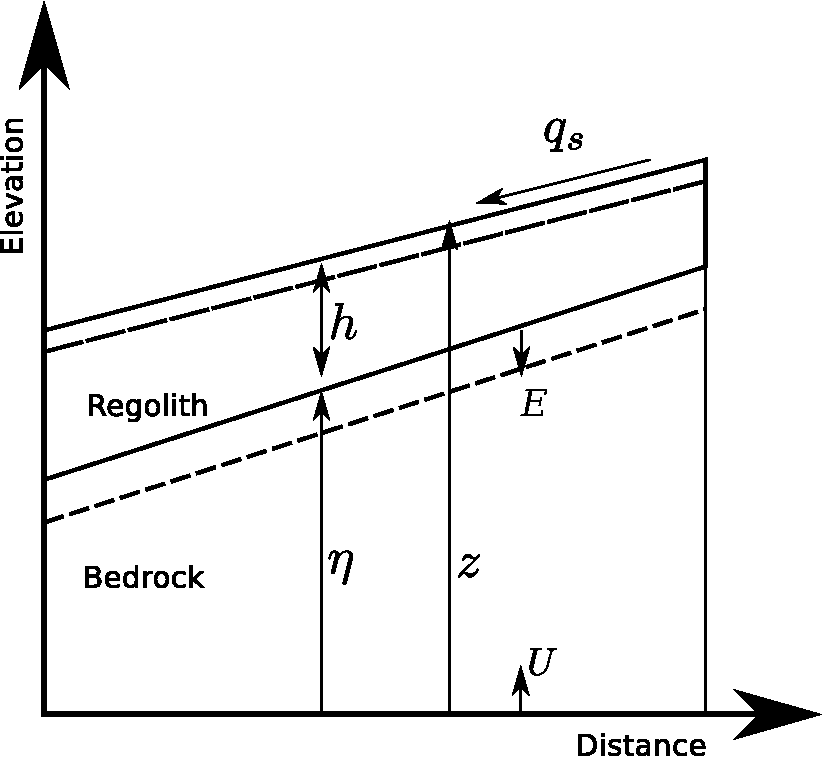
\includegraphics[width=8.6cm]{./figures/ch2-erosion-diagram.pdf}
\caption{Diagram showing the conservation of mass within a 2-D domain, where mass enters the system through uplift, $U$, and exists as sediment transported, $\mathbf{q}_{s}$ out of the domain. $E$ is the rate of production of regolith, $h$ is the thickness of regolith, $\eta$ is the bedrock elevation and $z$ is the total elevation.}
\label{fg:1dmodel}
\end{figure}

Following \cite{dietrich-etal-2003} I define a landscape of elevation $z$ composed of bedrock, thickness $\eta$, and a surface layer of sediment with thickness $h$ (Figure \ref{fg:1dmodel}). This landscape is forced externally through uplift rate $U$. The bedrock is transferred into sediment through erosion at a rate $E$ and the sediment is transported across the system with a flux $\mathbf{q}_{s}$. Assuming that the density of sediment and bedrock are equal, then the change in bedrock thickness is,
\begin{equation}
\frac{\partial\eta}{\partial t} = U - E,
\label{eq:bedrock}
\end{equation}
and the rate of change in sediment thickness is,
\begin{equation}
\frac{\partial h}{\partial t} = E - \nabla \cdot \mathbf{q}_{s}.
\label{eq:sediment}
\end{equation}
It then follows that the rate of change in landscape elevation is,
\begin{equation}
\frac{\partial z}{\partial t} = \frac{\partial\eta}{\partial t} + \frac{\partial h}{\partial t}.
\label{eq:elevation}
\end{equation}

To solve the mass balance I will make a strong assumption: there is always a supply of transportable sediment. Then I can follow through with the summation in equation \ref{eq:elevation} giving,
\begin{equation}
\frac{\partial z}{\partial t} = U - \nabla \cdot  \mathbf{q}_{s}.
\end{equation}
This may be appropriate when modelling the transport of sediment along the river bed and when considering the formation of alluvial fans \citep[e.g.][]{paola-etal-1992,whipple-2002,guerit-etal-2014}. In the absence of surface water we can assume that sediment flux is simply a function of local slope $\mathbf{q}_{s} = -\kappa\nabla z$. In the presence of flowing water then the sediment flux is a function of the flowing water and local slope $\mathbf{q}_{s} = -c\mathbf{q}_{w}^{\delta}\left(\nabla z\right)^{\gamma}$ where $c$ is the transport coefficient (units (m$^{2}$\,yr$^{-1}$)$^{1-\delta}$), $\mathbf{q}_{w}$ is the water flux per unit width, and the exponents $\delta > 1$ and $\gamma \geq 1$ are dependent on how sediment grains are transported along the bed \citep{smith-1972,paola-etal-1992}. Furthermore, $\delta > 1$ is required to create concentrated flow \citep{smith-1972}. The change in landscape elevation is then given by,
\begin{equation}
\frac{\partial z}{\partial t} = U + \nabla \cdot \left(\kappa\nabla z +c\mathbf{q}_{w}^{\delta}\left(\nabla z\right)^{\gamma}\right).
\end{equation}
which can be written as,
\begin{equation}
\frac{\partial z}{\partial t} = U + \nabla \cdot \left(\left[\kappa +c\mathbf{q}_{w}^{\delta}\left(\nabla z\right)^{\gamma-1}\right]\nabla z\right).
\label{eq:transport}
\end{equation}
Equation \ref{eq:transport} is non-linear in the case that $\gamma \neq 1$. In deriving this equation of elevation change due to sediment transport we have simply summed the two terms for sediment flux, the linear and potentially non-linear slope dependent terms. This summation has been done as it is the simplest way to generate landscape profiles that have the desired convex and concave elements observed in natural landscapes \citep{smith-1972}.

To solve this equation in one dimension I assume that the water flux is a function of the precipitation transported down the river network. The water collected is taken from the upstream drainage area, $a$, which is related to the main stream length, $l$, by $l \propto a^{h}$ where $h$ is the exponent taken from the empirical Hack's law \citep{hack-1957}. The main stream length is related to the longitudinal length of the catchment by, $l \propto x^{d}$ where $1 \leq d \leq 1.1$ \citep{tarboton-etal-1990,maritan-etal-1996}. Therefore, we can write that $x \propto a^{h/d}$, and the water flux is the precipitation rate, $\alpha$ units (m\,yr$^{-1}$), multiplied by the length of the drainage system,
\begin{equation}
q_{w} = k_{w}\alpha x^{p}
\label{eq:waterflux}
\end{equation}
where $k_{w}$ is the width coefficient (units m$^{1-p}$), and $p = d/h$. Furthermore it is observed that river catchments are typically longer than they are wide, and so $p<2$ \citep{dodds-2000a}. Therefore given that $0.5 < h < 0.7$ \citep[e.g.][]{rigon-etal-1996} then $1.4 < p < 2$, and the transport model (equation \ref{eq:transport}) becomes,
\begin{equation}
\frac{\partial z}{\partial t} = U + \frac{\partial}{\partial x} \left(\left[\kappa +ck_{w}\alpha^{\delta}x^{p\delta}\left(\frac{\partial z}{\partial x}\right)^{\gamma-1}\right]\frac{\partial z}{\partial x}\right).
\label{eq:1dtransport}
\end{equation}

\begin{figure}
\centering
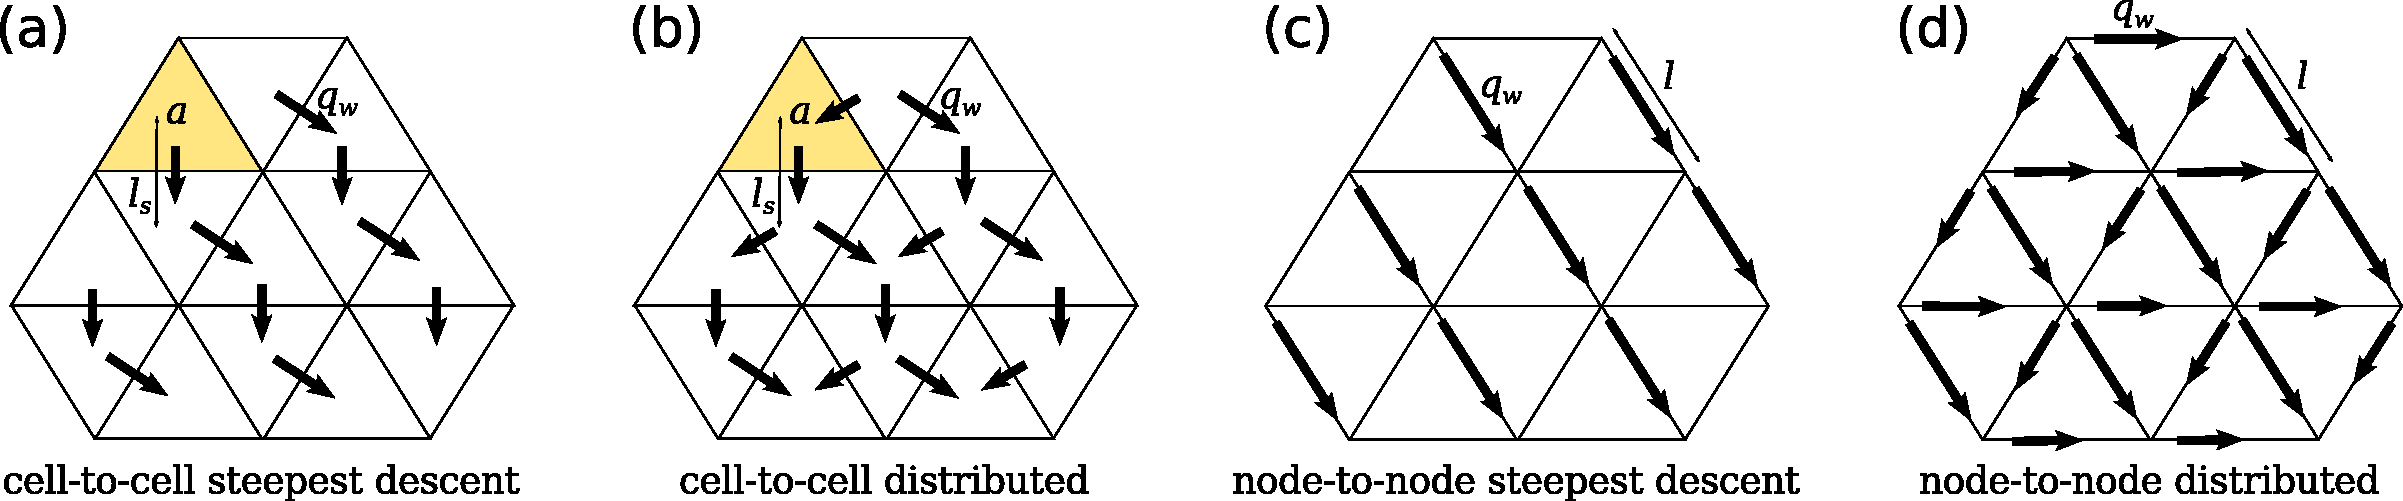
\includegraphics[width=\textwidth]{./figures/ch2-routing.pdf}
\caption{Diagram of flow routing from cell-to-cell and node-to-node for either a single flow direction (SFD) and a multiple flow direction (MFD) algorithm weighted by the relative gradient.}
\label{fg:routing}
\end{figure}

To solve equation \ref{eq:transport} over a 2-D domain requires an algorithm to route surface flow down the landscape. Water can be routed from cell-to-cell, where precipitation is collected over the area of each cell, sent downwards, and accumulates. In this cell-to-cell configuration the water flux has units of length squared per unit time and is given by:
\begin{equation}
q_{w}\mathrm{[cell]} = \frac{\alpha a}{l_{s}},
\label{eq:cell}
\end{equation}
where $\alpha$ is precipitation rate, $a$ is the cell area, and $l{s}$ is the length from cell centre to cell centre down the steepest slope (Figure \ref{fg:routing}a and b). This gives a water discharge per unit length, which has the advantage of not having to explicitly state the sub-grid width of the flow \citep{simpson-2003}. However, implicitly this implies that the flow is over the width of a cell. An alternative is to route water from node to node along cell edges and for it to accumulate. I assume that along the length of each cell edge water can be added to the flow line, assuming that the input is linearly related to the length of the flow line,
\begin{equation}
q_{w}\mathrm{[node]} = \alpha l,
\label{eq:node}
\end{equation}
where $l$ is the length of the edge that joins the up-slope node to the down-slope node (Figure \ref{fg:routing}c and d). This means that the cell area is ignored and instead water enters the flow path uniformly along its length and accumulates down slope.

Equation \ref{eq:node} makes the assumption that water accumulates as a function of length. Water flux is observed to related to catchment area, $Q_{w} \propto A^{0.8}$ \citep{syvitski-2007}. The catchment length, $l$ is then related to area by, $l\propto A^{1/p}$, where $1.4<p<2.0$ \citep{armitage-etal-esurf-2018}. At the lower end of the range this gives $Q_{w} \propto l^{1.12}$, suggesting that accumulating water as a linear function of flow length is a reasonable simplification. A knock on effect of this assumption is that the magnitude of the water flux predicted for the node-to-node routing is less than the cell-to-cell, as in the latter water is accumulated over cell areas, which is naturally larger than the cells edges.

Both equations \ref{eq:cell} and \ref{eq:node} do not attempt to capture the interaction between water flux and river width, rather these are two methods to approximate run-off within a coarse numerical grid. For both the cell-to-cell and node-to-node methods the flow can then be routed down a single flow direction (SFD) or routed down multiple flow directions (MFD) weighted by the relative gradient, as in for example \cite{schoorl-etal-2000}. The choice of flow routing has a large effect on the numerical solution. I showed that SFD creates a numerical solution that is highly resolution dependent \citep{armitage-2019}. It is only by using the MFD routing that model solutions are not resolution dependent (see code fLEM\footnote{fLEM: Fenics based Landscape Evolution Model, see \url{https://github.com/johnjarmitage/flem}}, Figure \ref{fg:MFD}, \citealp{armitage-2019}).

\begin{figure}
\centering
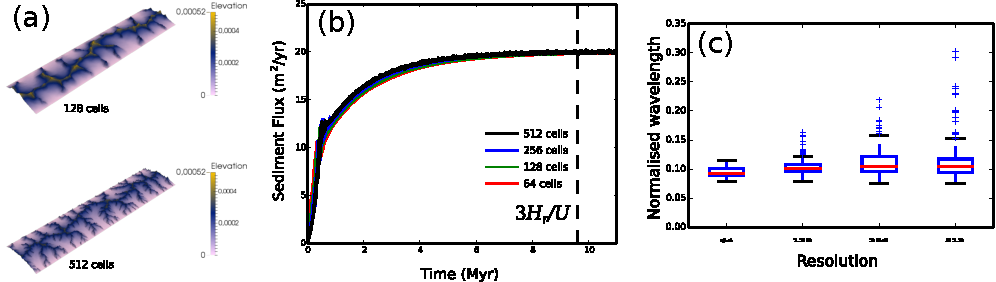
\includegraphics[width=\textwidth]{./figures/ch2-MFD.pdf}
\caption{A landscape evolution model fLEM \citep{armitage-2019}. (a) Dimensionless elevation from the node-to-node flow routing landscape evolution model with different flow routing algorithms at different numerical resolutions after a dimensionless run time of $1.563\times10^{-6}$ (5\,Myr), with an aspect ratio of $4\times1$. (b) Dimensional sediment flux that exits the model domain. (c) Box whisker plots of the dimensionless valley-to-valley wavelength for each model for different resolutions, where the number of cells along the y-axis is shown.}
\label{fg:MFD}
\end{figure}

The sediment flux generated by erosion within the model and the accommodation space generated by subsidence can be used to generate grain size profiles of the stratigraphic layers. The 1D down-system grain-size distribution is modified down-system by selective deposition following the theoretical model and observations of \cite{fedele-2007} and \cite{duller-etal-2010}. I assume perfect sorting, where only gravel is deposited until it is exhausted, followed by only sand and finally by fine-grained material (silt and clay grade; \citealp{paola-etal-1992}). Gravel undergoes fining according to an exponential function of Sternberg type \citep{fedele-2007,duller-etal-2010},
\begin{equation}
D(\tilde{x}) = D_{g0} + \phi_{0}\frac{1}{C_{v}}\left( e^{-C_{g}\tilde{y}}-1 \right).
\label{eq:fedele}
\end{equation}
The fining of the sand and smaller grain sizes is given by \cite{sternberg-1875},
\begin{equation}
D(\tilde{x}) = D_{si}e^{-C_{s}\tilde{y}}.
\label{eq:sternberg}
\end{equation}
In equations \ref{eq:fedele} and \ref{eq:sternberg} $\tilde{x}$ is the dimensionless down-system length, $D_{g0} = log_{10}\left(D_{50}\right)$ is the median of the gravel input taken from the 50th percentile from Wolman pebble-count data, $\phi_{0} = log_{10}\left( D_{84}/D_{50} \right)$ is the input variance of the gravel assuming that the distribution is log-normal, $D_{si} = log_{10}\left( 2\,{\rm mm} \right)$ is the initial grain-size for sand and finer material in the sediment input, and $\tilde{y}$ is the spatial transformation of the down-system distance given by \citep{paola-1995},
\begin{equation}
\frac{d\tilde{y}}{d\tilde{x}} = \frac{r}{q_{s}}
\end{equation}
where $r$ is the down-system distribution of deposition and $q_{s}$ is the down-system distribution of sediment discharge.

\end{subappendices}
